\begingroup
\clearpage% Manually insert \clearpage
\let\clearpage\relax% Remove \clearpage functionality
\vspace*{-16pt}% Insert needed vertical retraction
\chapter[OBJECT RECONSTRUCTION AND EVENT SIMULATION IN ATLAS]{OBJECT RECONSTRUCTION AND EVENT SIMULATION IN ATLAS}
\label{ch4}
\endgroup

The previous chapter went into detail on how the \gls{atlas} detector works through its various sub-detectors and and systems. Collisions occur at the beam axis, creating a shower 
of particles into the detector, depositing energy on an object's corresponding detector and having its tracks mapped by several systems within the \gls{id}. These recorded signals 
from \textit{triggered} events are used to reconstruct the event using complex algorithms. 
\par
Figure 18 shows a slice of the \gls{atlas} sub-detectors with several different objects from a single event depositing energy in corresponding sensors. The trajectories 
of charged particles (tracks) are reconstructed using the \gls{id} \cite{atlas}. Muons are reconstructed using associated tracks measured within the muon spectrometer and 
tracks left within the \gls{id} \cite{muon-reco}. Electrons are reconstructed using tracks detected within the \gls{id} along with energy deposits within the \gls{ecal} \cite{e-y_performance}.
Photons will also deposit their energy within the \gls{ecal}, but do not leave any tracks, thus being able to separate both electromagnetic objects. 
\par
From these collision events are objects known as jets, i.e., hadron cones due to hadronization of quarks and gluons as seen in Figure \ref{fig:4.1} as the red deposits in the blue \gls{hcal}.
Due to hadronization, multiple tracks are associated with jets which is why jets are reconstructed and not individual hadrons. Jets can be caused by several different hadrons 
and so we separate these types into, what we call, flavors. Jets caused by \textit{b}-hadrons are called \textit{b}-jets, and likewise, \textit{c}-hadrons cause \textit{c}-jets. 
The lighter quarks (up, down and strange as discussed in Section \ref{sect:standard_model}) are difficult to differentiate due to their similar size in mass. We group these hadrons 
into a single category of jets called \textit{light}-jets. As jets propagate outward they create a cone like shape within the \gls{hcal}, covering an angular 
area. Jets that cover a large angular area are considered large-radius jets \cite{large-r-jets} which contain interesting physics and are a focused object for the preliminary 
analysis in the last chapter of this thesis. 

\begin{figure}[h]
    \centering
    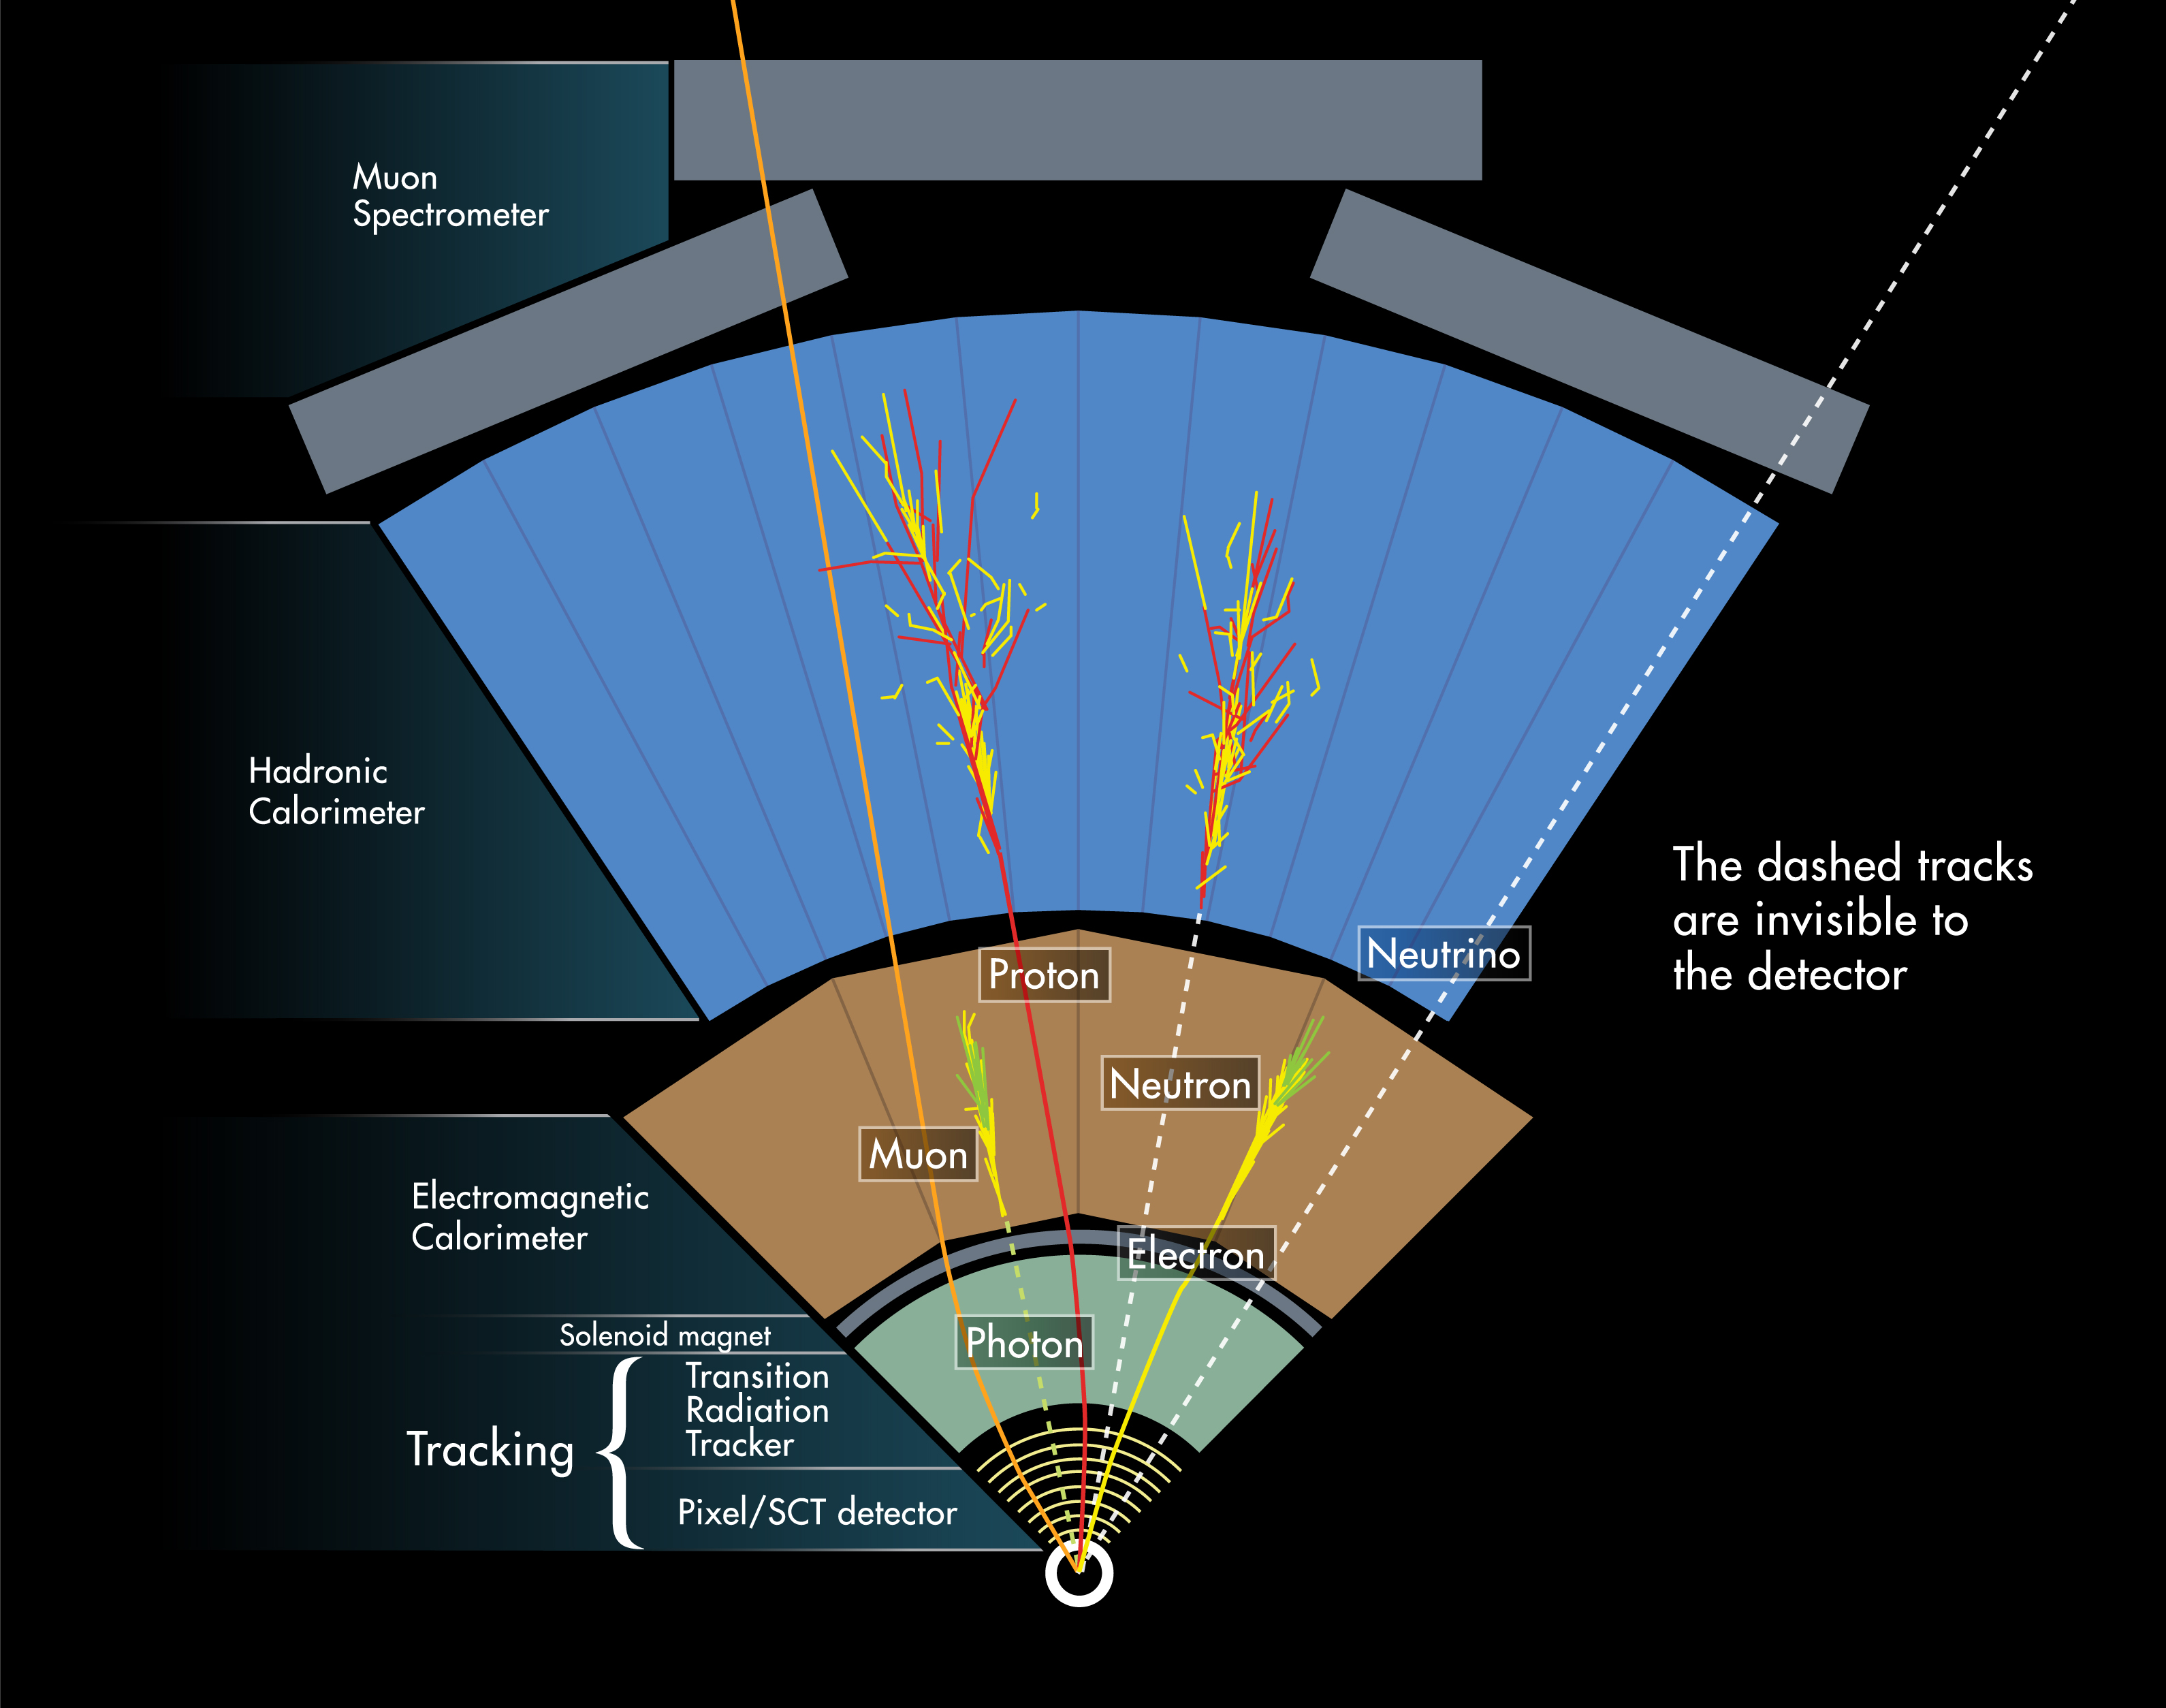
\includegraphics[scale=0.6]{figs/ch4/ATLAS-tracks.jpg}
    \caption{ Planar slice of the ATLAS detector showing different energy deposits of several physics objects \cite{atlas-detects}.}
\label{fig:4.1}
\end{figure}

\section{Track and Vertex Reconstruction}\label{sec:track-reco}

Almost all physics objects detected by \gls{atlas} deposit small amounts of energy within the \gls{id} sensors, each \textit{hit} is then used to reconstruct the object's 
track(s). Tracks are seeded by groups of three, one from the \gls{ibl}, another from the pixel detector and lastly the \gls{sct} \cite{track-reco}. Within the pixel and \gls{sct}
detectors, the track association begins with clustering raw measurements. A connected component analysis (\gls{cca}) \cite{cca} groups pixels and strip detectors together that share
a common edge or corner if energy has deposited on them above a certain threshold. These combined clusters are then referred to as \textit{space-points}. The average size of a
pixel cluster is about 2 pixels in the \textit{r}-$\phi$ plane and 1 to 3 pixels in the longitudinal direction with increasing η. Clusters from single charged particles are 
\textit{single-particle} clusters, clusters from multiple charged particles are referred to as \textit{merged} clusters and clusters from multiple tracks that are not 
compatible are called \textit{shared} clusters. A Kalman filter \cite{kalman} is applied to these \textit{merged} 
clusters to maximize track purity for objects of interest. Particles often share a hit, in this case a quality score is assigned to each track candidate. The score is 
determined by the number of \gls{id} layers with a hit, a track fit $\chi^{\textrm{2}}$ and the logarithm of the track momentum to suppress low $\textit{\textit{p}}_{\textrm{T}}$ 
track objects \cite{track-reco,newt}. For clusters assigned to multiple tracks in the merged clusters category, an ambiguity solver is applied. For the track selection criteria,
a track cannot be associated to no more than two shared clusters, cannot be over $\textit{\textit{p}}_{\textrm{T}} > \textrm{400 MeV}$ and $|\textrm{η}| < \textrm{2.5}$.
Using the hits in the \gls{trt}, the final track candidates are mapped out and a final selection occurs through track fitting. 
\par
Through the multiple \gls{pp} collisions in a bunch crossing, there is typically a single collision that yields objects of interest, this is called the hard-scatter. 
The main vertex of the hard-scatter and the secondary vertices from its decay products are mapped through the tracking procedure by applying track criteria. Multiple vertices
are found on the \textit{z}-axis from luminous peaks, called seed vertices. Here is where the track algorithm and its criteria are applied to find the primary vertex 
of the hard-scatter.

\section{Electrons}\label{sec:ele-reco}

Electrons are reconstructed using the energy deposits within the \gls{ecal} and tracks within the \gls{id}. The reconstruction comes in several steps. The first is combining the 
energy clusters within the \gls{ecal} into \gls{em}-topo clusters. Tracks are then matched to these clusters, creating superclusters. Electrons are then defined from these 
superclusters \cite{ele-reco}. 
\par
Proto-clusters are first defined within the \gls{ecal} and \gls{hcal} using a set of noise thresholds to discriminate from background noise. The clusters found in the \gls{hcal}
are not used in the electron reconstruction process, but are used to reduce background noise from pile-up. The cell clusters are required to 
have a significance $|\zeta^{\textrm{EM}}_{\textrm{cell}}| \ge \textrm{4}$ as defined in Eq. \ref{eq:4.1} \cite{ele-reco}:
%
\begin{equation}\label{eq:4.1}
    \zeta^{\textrm{EM}}_{\textrm{cell}} = \frac{\textrm{\textit{E}}^{\textrm{EM}}_{\textrm{cell}}}{\sigma^{\textrm{EM}}_{\textrm{noise,cell}}} 
\tag{4.1}
\end{equation}
%
$\textrm{\textit{E}}^{\textrm{EM}}_{\textrm{cell}}$ is the cell energy deposition and $\sigma^{\textrm{EM}}_{\textrm{noise,cell}}$ is the expected cell noise. This noise is 
the known electronics noise and an estimate of the pile-up noise corresponding to the instantaneous luminosity of Run 2. The algorithm then iterates through these clusters,
ignoring the first of the \gls{ecal} in order to suppress noise. These proto-clusters are then paired with neighboring clusters with a significance of $|\zeta^{\textrm{EM}}_{\textrm{cell}}| \ge \textrm{2}$.
These neighbors are then used as seed clusters of the next iteration to further find neighboring cells within the cluster. Once all the neighboring clusters with
$|\zeta^{\textrm{EM}}_{\textrm{cell}}| \ge \textrm{2}$ are found, they are then merged into a larger cluster. Proto-clusters with more than two or more local energy maxima, 
they are split into separate clusters. A maxima is considered when it has $\textrm{\textit{E}}^{\textrm{EM}}_{\textrm{cell}} >$ 500 MeV and at least four neighbors with 
smaller signal.   
\par
Tracks are then matched to the proto-clusters using information from the \gls{id} as described in Section \ref{sec:track-reco} \cite{ele-reco-2015}. Electrons lose a significant portion of their energy 
within the \gls{id} compared to other charged particles. To ensure efficiency in electron reconstruction, a loose track association criteria is applied. The conditions are 
$|\textrm{η}_{\textrm{track}} - \textrm{η}_{\textrm{cluster}}| <$ 0.05 and $-\textrm{0.10} < \textrm{\textit{q}}(\phi_{\textrm{track}} - \phi_{\textrm{cluster}}) <$ 0.05 where 
\textit{q} refers to the charge of the track. An ordering is applied to cases when multiple tracks are matched to a single cluster. Tracks found in the pixel detector are the most 
preferred, then tracks within the \gls{sct} with none in the pixel detector. Then the best $∆\mathrm{\textrm{R}}$ between the tracks and the cluster chosen. The track with the best score 
is then matched to the \gls{ecal} cluster and is used in the further steps of electron reconstruction.
\par
Superclusters are then defined from these chosen \gls{em} topo-clusters. The seeds chosen to form the superclusters are selected by requiring 
$\textit{E}_{\textrm{T}} = \sqrt{\textrm{\textit{m}}^{\textrm{2}}+\textit{\textit{p}}_{\textrm{T}}^{\textrm{2}}} \ge$ 1 GeV and matched track fulfilling quality criteria.
These superclusters are then extended by adding topo-clusters within $∆\textrm{η} \times ∆\phi =$ 0.075 $\times$ 0.125, these are considered \textit{satellite} clusters 
and are assumed to be secondary \gls{em} showers from the initial electron or photon. But for electrons, this distance is extended to $∆\textrm{η} \times ∆\phi =$ 0.125 $\times$ 0.3
 and the seed and the adjacent topo-cluster must share a matched track. These steps rely heavily on tracking information to discriminate between radiative photons or low energy 
 electrons from pile-up or noise. 
 \par
Once the superclusters are built, an initial energy calibration and position correction are applied to them. Tracks are matched to these supercluster while conversion vertices 
are matched to photons since they do not leave tracks within the \gls{id}. There are events with clear cut identification of electrons and photons, i.e., superclusters with 
defined tracks (electrons) and superclusters with no defined tracks (photons). But there are cases when there is ambiguity between both objects, when this occurs a classification 
process is applied to determine the type of object. The initial suepercluster calibration occurs before the track matching and relies on energy calibrations of the
electrons and photons to simulations \cite{ele-cali}. This process is referred to as energy scale calibration. The energy resolution of electrons found in data are used 
to calibrate simulations of $\textrm{\textit{Z}} \rightarrow \textrm{\textit{ee}}$ events. These simulated events are then used to derive the energy scale and resolution calibration 
factors. The invariant mass of two electrons in data and within these simulated events after the energy resolution is applied can be found in Figure \ref{fig:4.2} with good agreement.

\begin{figure}[h]
    \centering
    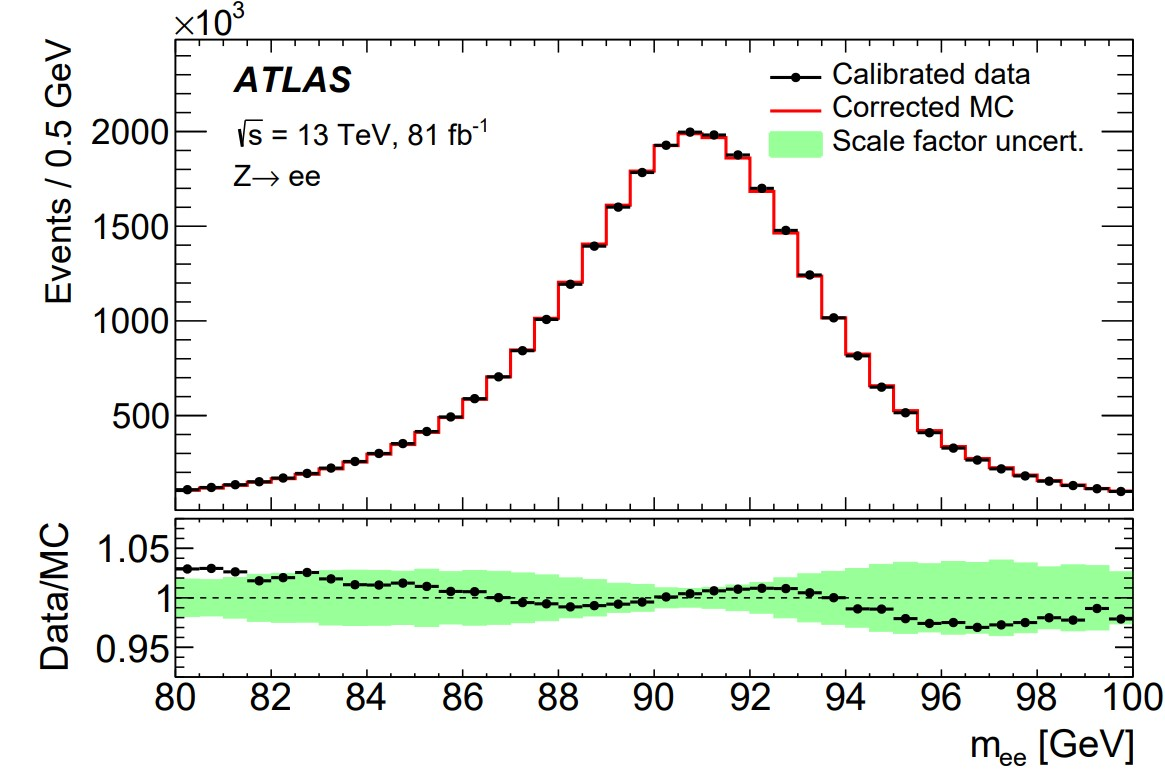
\includegraphics[scale=0.38]{figs/ch4/JES-ele.jpg}
    \caption{ Comparisons of simulated events and data after calibration and resolution corrections applied for electrons \cite{ele-reco}.}
\label{fig:4.2}
\end{figure}

\section{Muons}\label{sec:muon-reco}

Muons deposit little energy as it transverses the \gls{atlas} detector, thus its reconstruction relies heavily on associated tracks left within the \gls{id} and the (\gls{ms}) 
along with characteristic energy deposits in the calorimeters. The track reconstruction is for the \gls{ms} is independent of the track reconstruction in the \gls{id} as described 
in section \ref{sec:track-reco}, though the reconstructed muon depends on both \cite{muon-reco}.
\par  
Tracks within the \gls{ms} are identified as short straight-line local segments reconstructed from hits in individual stations. These segments are identified through a process 
known as a Hough transform \cite{Hough}. These segments are combined into preliminary track candidates using a loose constraint of the impact parameter (\gls{ip}, discussed in Section~\ref{sec:ip-algo}) and a parabolic trajectory that includes the first-order approximation of the track bending due to the magnetic field. These calculations are combined with precision 
information of a second coordinate from the trigger detectors, creating a three-dimensional track. This track then has a global fit $\chi^{\textrm{2}}$ fit of the muon trajectory
through the magnetic fields within the \gls{ms}. The hits that are not contained within the fit of the muon trajectory are removed. Hits are added onto the fit trajectory that 
were not originally there, from these aligned hits, another $\chi^{\textrm{2}}$ fit is applied. Less quality tracks are removed when they share a fraction of hits with a high 
quality track in order to resolve ambiguities. The final track is then re-fitted with a \gls{ip} constraint that takes into account the energy loss in the calorimeters and 
an extrapolated trajectory back to the beam line \cite{muon-reco}. 
\par
This fitting procedure using hits within the \gls{ms} and \gls{id} are applied in several different reconstruction strategies.

\begin{itemize}
    \item Combined (CB): Combined muons are identified by matching \gls{ms} to \gls{id} tracks and applying a combined fit as previously discussed. For muons with 
    $|\textrm{η}| >$ 2.5, \gls{ms} track segments are combined with hits from the pixel detector and \gls{sct} detector. These boosted muons are considered a subset called 
    silicon-associated forward (SiF) muons
    \item Inside-Out Combined (IO): Muons reconstructed using this method uses an algorithm which extrapolates the \gls{id} hits to the \gls{ms} and searches for at minimum three
    loosely associated hits. Between these loosely associated hits, the small energy loss within the calorimeters are used to verify. A Combined track fit is then applied.
    \item Muon-Spectrometer Extrapolated (ME): These are muon tracks within the \gls{ms} but cannot be associated with any hits within the \gls{id}. If this is the case, the tracks
    are extrapolated all the way back to the beam line. Because of this, this extends the \gls{ms} coverage to $|\textrm{η}| =$ 2.7.  
    \item Segment-Tagged (ST): ST requires at least one \gls{ms} segment to be associated with an extrapolated \gls{id} track. 
    \item Calorimeter-Tagged {CT}: These muons are identified by taking the extrapolated tracks in the \gls{id} through the calorimeters. Muons deposit minimum-ionizing 
    energy in the calorimeters. If CT was used to identify the muon, the parameters are obtained directly through the track fit. 
\end{itemize}

After reconstruction, high quality muon candidates are then selected using criteria utilizing the sub-detectors. The set of requirements on the identified muons given its type as 
stated above is referred to as its selection \textit{working point} (\gls{wp}). The definition of muon \gls{wp}s depends on the type of analysis involving final state muons. 
The standard \gls{wp}s designed to cover needs of most analyses vary in increasing purity and decreasing muon tagging efficiency. The \gls{wp}s are \textit{loose}, \textit{medium},
and \textit{tight}. Here, muons passing the \textit{medium} \gls{wp} is a subset of the \textit{loose} \gls{wp}. These were defined to help optimize different physics analyses. 
The \textit{medium} \gls{wp} is suitable for most general analyses where the \textit{loose} was optimized for Higgs boson decays into a four muon final state \cite{muon-reco}.
\par
Muon correction factors are obtained through simulation events of $\textrm{\textit{Z}} \rightarrow \textrm{\textit{µµ}}$ and $\textrm{\textit{J}}/\psi \rightarrow \textrm{\textit{µµ}}$. The momenta
in the simulation are corrected to those obtained through data. Multiplicative correction factors are obtained to correct for reconstruction, identification, and isolation 
efficiencies of simulation to data. 

\section{Jets}

Most \gls{pp} collision events result is quarks or gluons. Due to quark confinement within \gls{qcd}, these partons cannot exist independently and undergo 
a process called hadronization, resulting in color-less cone-like sprays of hadrons. The cones, or jets, are reconstructed using tracks from the \gls{id} and energy 
depositions with the \gls{hcal}. The energy deposition and correlated tracks undergo the same topo-cluster algorithm defined for electrons that was discussed in section \ref{sec:ele-reco}.
Two types of jets are defined depending on the radii of the cone. There are small-radius (\gls{sr}) jets and large-radius (\gls{lr}) jets.
Figure \ref{fig:4.1} shows two jets deposited in the blue colored \gls{hcal}, one from a proton, the other from a neutron. 

\subsection{Jet Definition}\label{sec:jet-def}

Since quarks cannot exist independently due to quark confinement, jet reconstruction must rely on complex algorithms exploiting jet kinematics in order to identify the 
initial quark. The jet reconstruction algorithm must allow for reliable comparison to theory and experiment \cite{antikt}. In order to identify jets associated to the hard-scatter 
event, the jet algorithm must be insensitive to soft (low momentum) and collinear (low angle) hadrons. 
\par
The current \gls{atlas} standard of such algorithms is called the anti-$\textrm{\textit{k}}_{\textrm{T}}$ algorithm \cite{antikt}. This process identifies hadronic energy depositions as inputs and forms 
jets through sets of criteria. First it chooses some object \textit{i} in a list of objects, calculates the distance $\textrm{d}_{\textrm{\textit{i}}\textrm{\textit{j}}}$
between two objects within the list and then it calculates the distance $\textrm{d}_{\textrm{\textit{i}}\textrm{\textit{B}}}$ between object \textit{i} and the beam (\textit{B}).
This is shown in Eq. \ref{eq:4.2} .
%
\begin{equation}\label{eq:4.2}
\begin{split}
    \textrm{d}_{\textrm{\textit{i}}\textrm{\textit{j}}} = \textrm{min}(\textrm{\textit{p}}^{\textrm{2\textit{p}}}_{\textrm{T,\textit{i}}},\textrm{\textit{p}}^{\textrm{2\textit{p}}}_{\textrm{T,\textit{j}}}) \frac{∆^{\textrm{2}}_{\textrm{\textit{i,j}}}}{\textrm{R}^{\textrm{2}}} \ ,\\
    \textrm{d}_{\textrm{\textit{i}}\textrm{\textit{B}}} = \textrm{\textit{p}}^{\textrm{2p}}_{\textrm{\textit{ti}}}
\end{split}
\tag{4.2}
\end{equation}
%
Where:
%
\begin{equation}\label{eq:4.3}
    ∆^{\textrm{2}}_{\textrm{\textit{i,j}}} = (\textrm{\textit{y}}_{\textrm{\textit{i}}}-\textrm{\textit{y}}_{\textrm{\textit{j}}})^{\textrm{2}} + (\phi_{\textrm{\textit{i}}}-\phi_{\textrm{\textit{j}}})^{\textrm{2}}
\tag{4.3}
\end{equation}
%
and $\textrm{\textit{p}}_{\textrm{T,\textit{i}}}$, \textit{y}$_{\textrm{\textit{i}}}$ and $\phi_{\textrm{\textit{i}}}$ are respectively the momentum, rapidity, and azimuthal 
angle of object \textit{i}. The radius of the jet cone is denoted as \textit{R} and the parameter \textit{p} is to help govern relative power of the energy. For the anti-$\textrm{\textit{k}}_{\textrm{T}}$ 
algorithm the parameter \textit{p} is set to $-$1. The algorithm then finds the minimum between $\textrm{d}_{\textrm{\textit{i}}\textrm{\textit{j}}}$ and $\textrm{d}_{\textrm{\textit{i}}\textrm{\textit{B}}}$.
if the minimum is the distance between the two objects \textit{i} and \textit{j}, then the four momenta of the objects are combined. Whereas, if the  $\textrm{d}_{\textrm{\textit{i}}\textrm{\textit{B}}}$
is the minimum, object \textit{i} is regarded as a jet. This procedure continues as long as objects remain on the list. 
\par
Due to the inverse dependence on $\textrm{\textit{p}}_{\textrm{T}}$, soft objects are combined with close-by hard objects (high momentum) before two soft objects are combined \cite{antikt}.
Jets tend to have a conical shape around the hardest object \textit{i} when using anti-$\textrm{\textit{k}}_{\textrm{T}}$ algorithm for reconstruction. However, when two hard objects are within a relative 
distance of $∆(\textit{i},\textit{j}) \le \textrm{2}\textrm{R}$ of one another, it's difficult to differentiate the jet substructure of either jet. If the two hard objects are within 
$\textrm{R} < ∆(\textit{i},\textit{j}) \le \textrm{2}\textrm{R}$ then the anti-$\textrm{\textit{k}}_{\textrm{T}}$ algorithm forms two jets. The shapes of these two hard object jets depends on the transverse 
momenta of both, ending in one shape to be conical where the other is partially cone-shaped. If two hard objects are found within $∆(\textit{i},\textit{j}) < \textrm{R}$, a single 
jet is formed and the shape is defined by the momenta of the two hard objects. If the momenta are similar, the jet is can be constructed of two cones (with radii lower than R)
inside one larger cone. Figure \ref{fig:antikt} shows several jets classified using the anti-$\textrm{\textit{k}}_{\textrm{T}}$ algorithm, along with a large-radius jet containing two small-radius jets. 
\par 
Two types of jets are presented in this thesis. Both are the previously stated \gls{sr} and \gls{lr} jets. The cone radii for these types correspond to R = 0.4 for \gls{sr} and 
R = 1.0 for \gls{lr}. More about these two types are explained in the following sections.

\begin{figure}[H]
    \centering
    \subfloat[\centering ]{{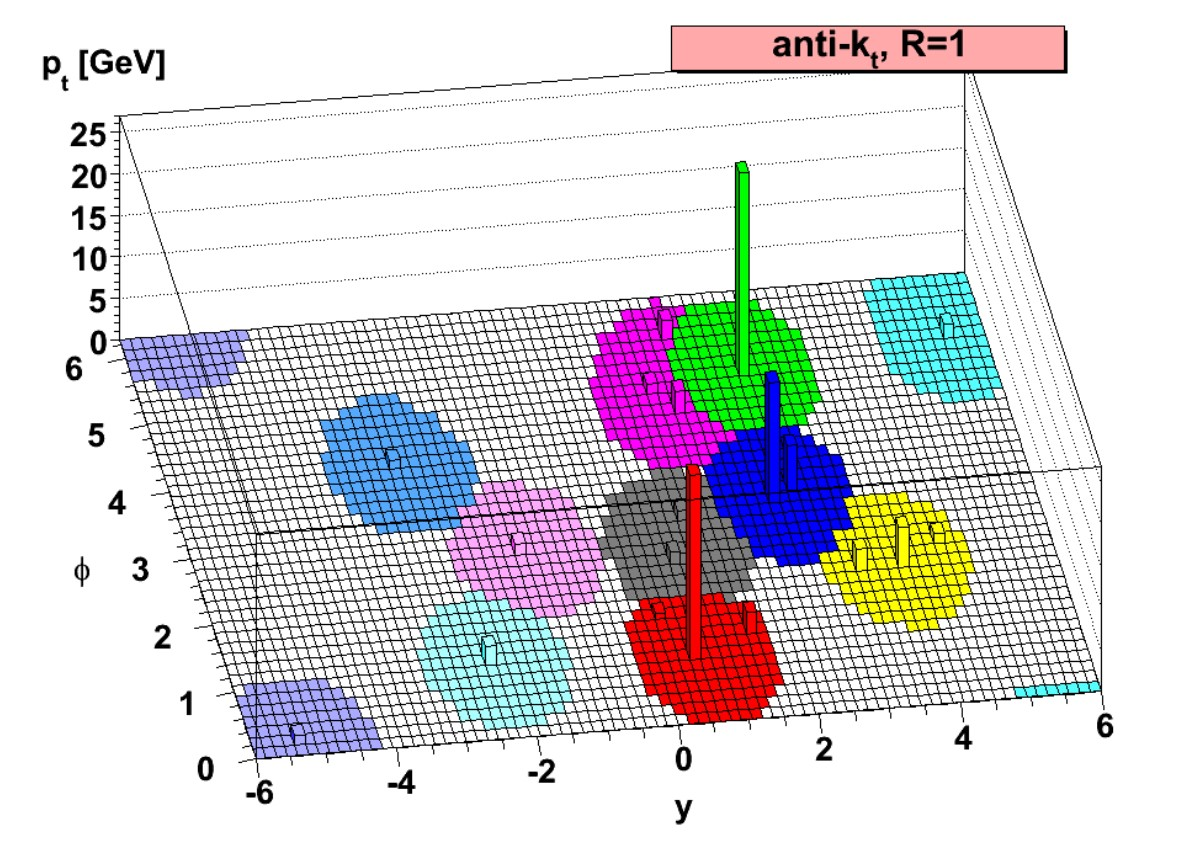
\includegraphics[scale=0.25]{figs/ch4/antikt.jpg}}}%
    \qquad
    \subfloat[\centering ]{{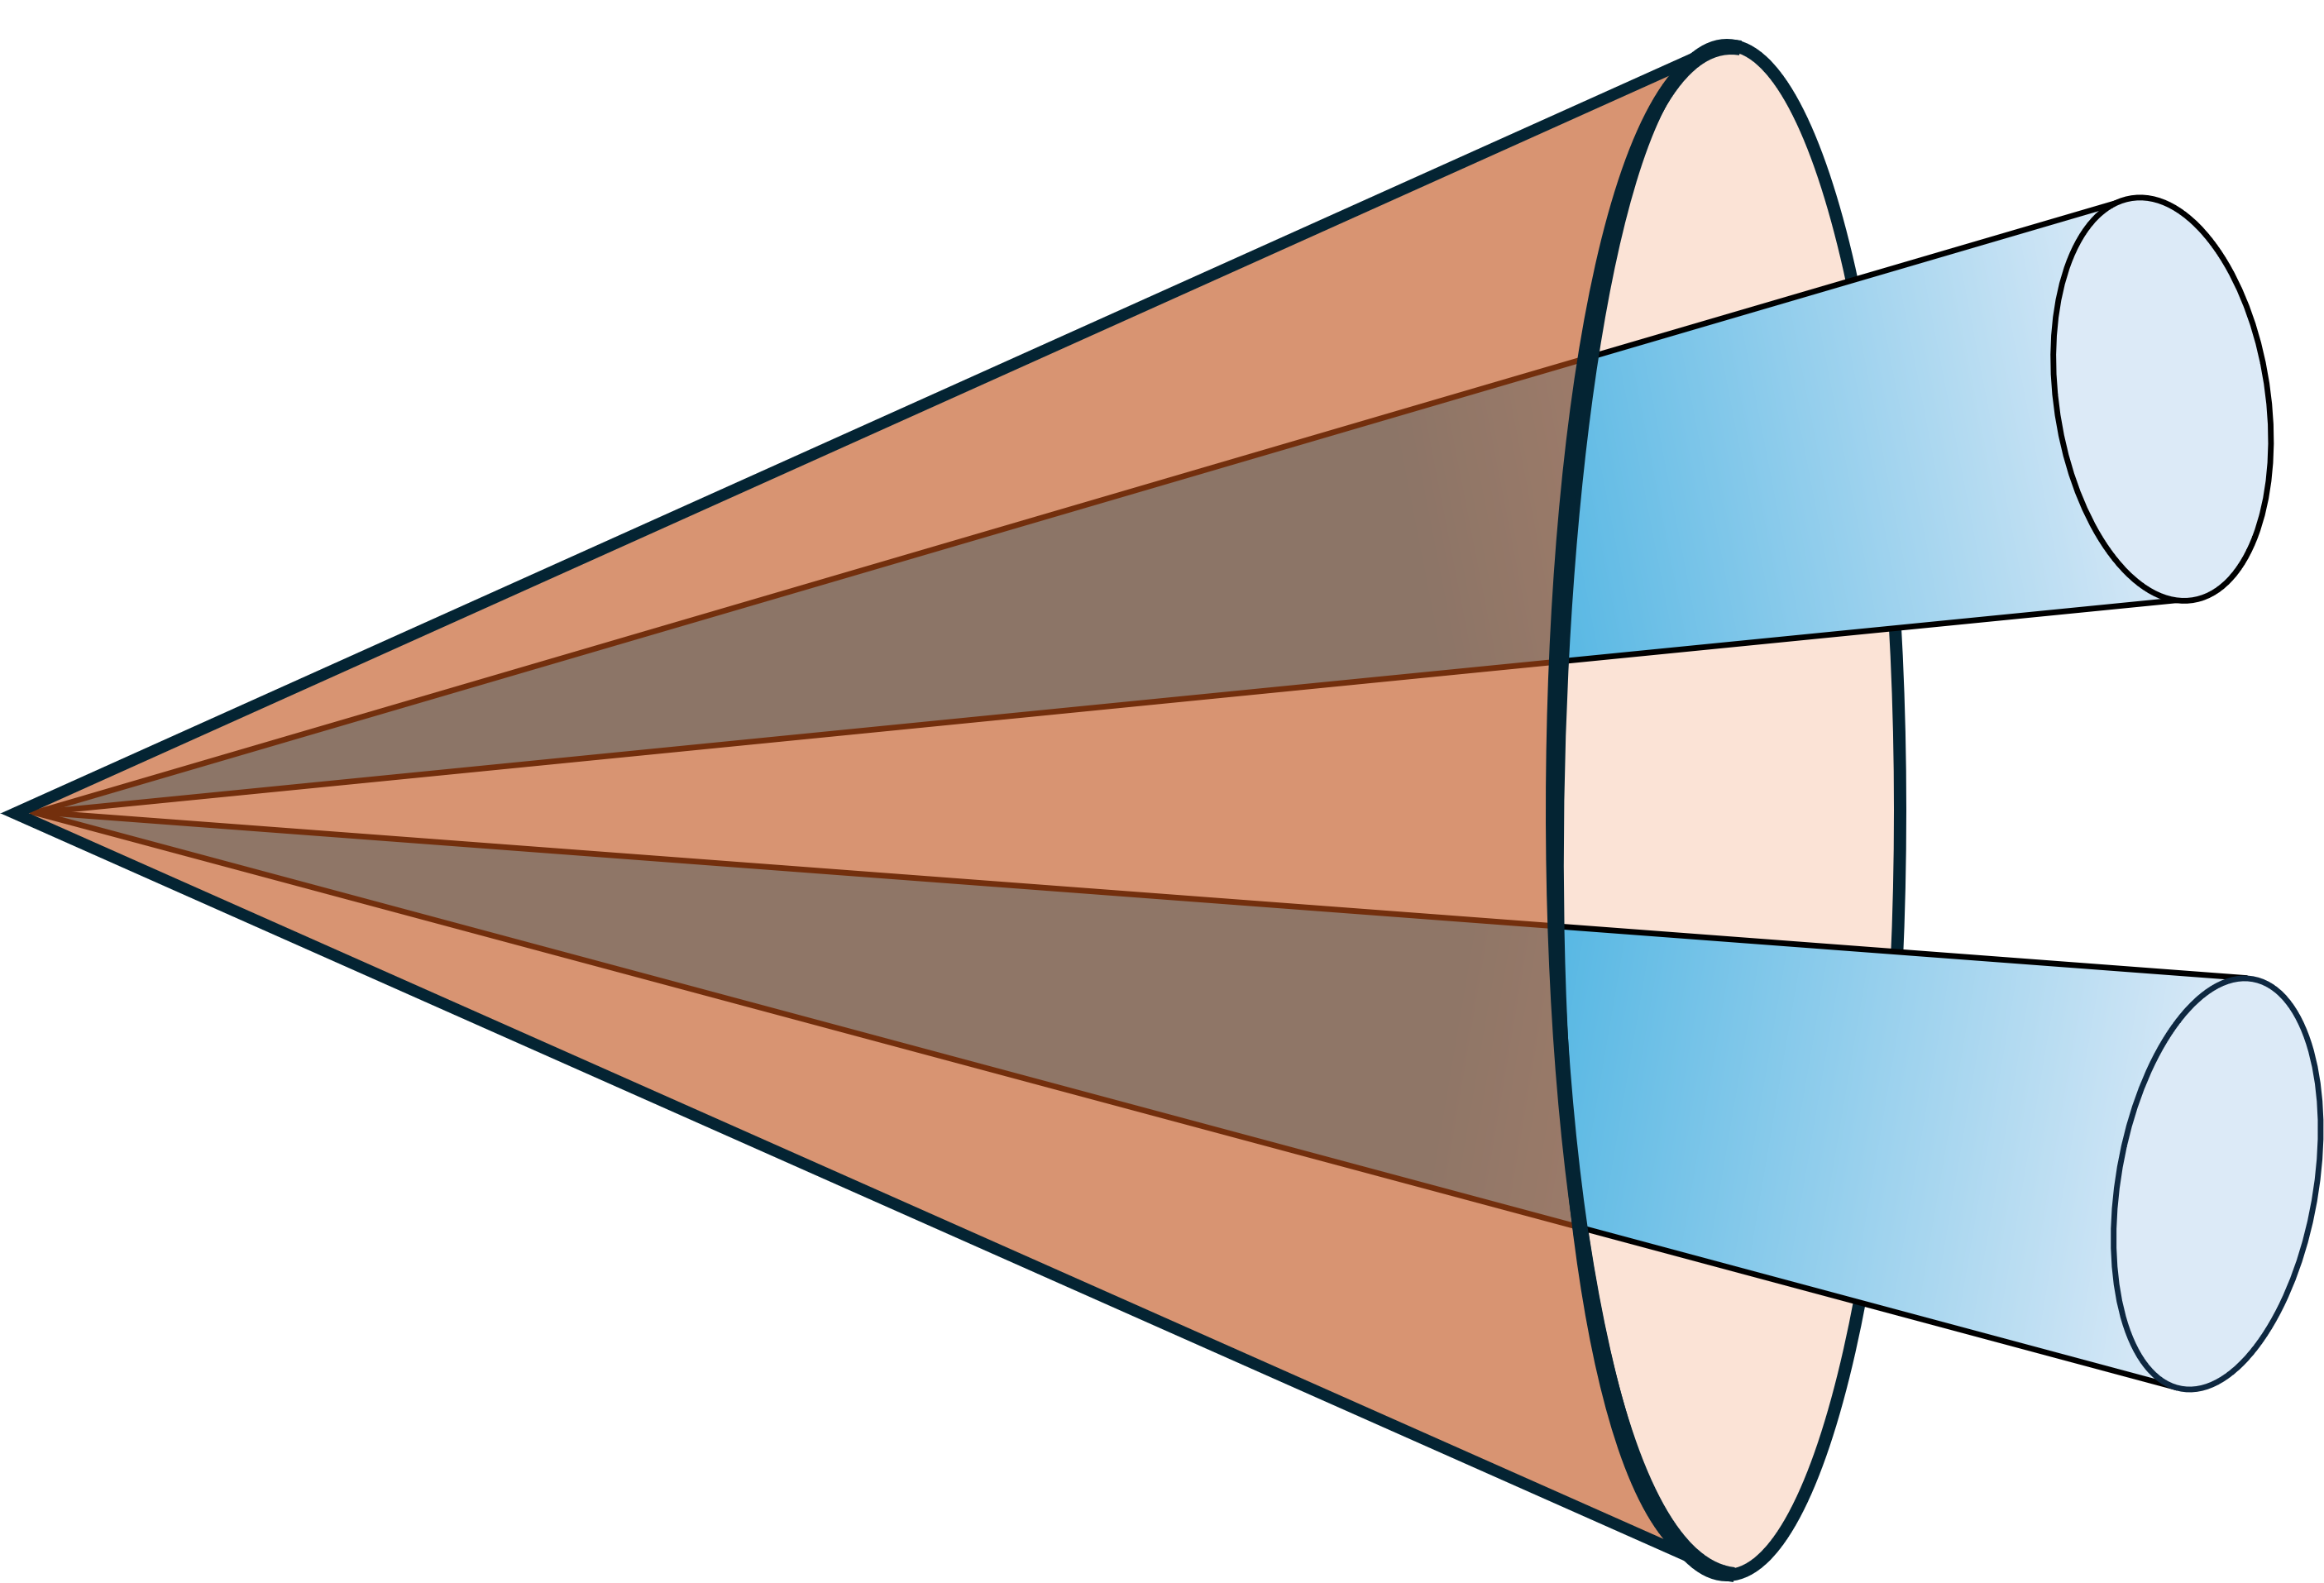
\includegraphics[scale=0.25]{figs/ch4/LR_jet.png}}}%
    \caption{(a) Shapes and the substructures of jets formed using the anti-$\textrm{\textit{k}}_{\textrm{T}}$ algorithm in the $\phi$ -\textit{y} plane \cite{antikt}. The height in the \textit{z}-axis corresponds to the momentum of the hard objects. 
    Figure (b) Substructure of a large-radius jet containing two small-radius jets of similar $\textrm{\textit{p}}_{\textrm{T}}$ }
    \label{fig:antikt}
  \end{figure}

\subsection{Small Radius Jets}\label{sec:small-R}

There are several approaches to defining a \gls{sr} jet. The jets used in this thesis, and are currently ATLAS standard objects, are called \textit{particle flow} or \textit{PFlow}.
PFlow objects are the building blocks of PFlow jets. These objects are clusters within the calorimeters and their constituted tracks \cite{pflow,jes}. Proto-clusters as previously defined in 
Section \ref{sec:ele-reco} are standard PFlow objects \cite{ele-reco}. The energy depositions in the \gls{ecal} and \gls{hcal} used to form these proto-clusters are calibrated 
to the \gls{em} scale in order to get a correct measurement of the showers \cite{jes}. A weighted mean of the cluster cells is calculated. This value is used to assign 
$\phi$ and η coordinates, as well as the energy deposited \cite{topo-cluster}. From here, it's assumed this cluster points to the origin of the coordinate system of the detector.
The proto-cluster is taken as a particle of zero mass and has its four-momentum calculated \cite{topo-cluster}. All the weighted clusters are assumed to be produced from objects
originating from the hard-scatter, an origin correction is then applied \cite{jes}, altering the momentum values to point towards the primary vertex. 
\par
\gls{sr} are defined as these corrected calorimeter proto-clusters with their associated tracks. A previously used jet class called \textit{EMTopo} jets was used. But this class 
only utilized the proto-cluster energy depositions and didn't use the track information from the \gls{id}. The \gls{id} has very precise momentum resolution for low 
momentum tracks, combining these to the calorimeter energy depositions greatly increased jet energy resolution in low energy jets. Giving jets improvements in its energy and 
direction while also lessening dependence on the number of pile-up interactions \cite{jes}.
\par
Tracks defined as PFlow objects but adhere to a tighter criteria than previous cases. A crucial energy subtraction procedure is performed to prevent double counting of energy 
contributions of charged particles leaving tracks in the \gls{id} and energy deposited in the calorimeters \cite{pflow,jes}. Energy that can be associated to a PFlow track is 
subtracted out of the clusters. A distance metric is applied between the center of the cluster and its possibly associated track as defined in Eq. \ref{eq:4.4}.

\begin{equation}\label{eq:4.4}
    ∆\textit{R'} = \sqrt{\left(\frac{∆\phi}{\sigma_{\phi}}\right)^{\textrm{2}}+\left(\frac{∆\textrm{η}}{\sigma_{\textrm{η}}}\right)^{\textrm{2}}}
\tag{4.4}
\end{equation}

Where $\sigma_{\phi}$ and $\sigma_{\textrm{η}}$ represent the angular topo-cluster width, calculated as the standard deviation of the displacements, $\phi$ and $\textrm{η}$, of the 
cluster cell center \cite{pflow}. Taking the smallest $∆\textit{R'}$ to be matched to a track succeeds in virtually 
all particles with $\textrm{\textit{p}}_{\textrm{T}} >$ 5 GeV. If no topo-cluster is found in a cone with $∆\textit{R'}$ = 1.64, it is assumed the particle did not form a cluster 
in the calorimeter and no momentum procedure is applied \cite{pflow}. 
\par
For each track matched to a cluster, the energy deposited by the particle is evaluated using simulated events. After a charged particle traversed the \gls{id}, it is possible that 
it would leave more than one topo-cluster in the calorimeters. If this is the case and the topo-cluster has energy below the expected amount, clusters within $∆\textit{R'}$ = 0.2
of the track are combined. Once the track-to-cluster matching occurs, energy is subtracted from the calorimeter topo-clusters. Energy deposits around the subtracted clusters 
that are found within reasonable shower fluctuations are also subtracted. The final PFlow object is considered the total subtracted energy from the calorimeter and the matched 
tracks that are compatible to the primary vertex. 

\subsection{Large Radius Jets}

As the momentum of massive particles (e.g. W, Z, Higgs, or the top-quark) increases, they become more Lorentz boosted. When these particles decay, their decay products are also 
highly Lorentz boosted, collimating them in a single direction. It is advantageous, in this case, to adjust the radius parameter \textit{R} from the small-R jets and to increase it in 
order to contain all the collimated decay products. The parameter for large-R jets is increased to \textit{R} = 1.0. By increasing the radius parameter, multi-pronged jet 
substructure from two-body or three-body decays is much more effectively captured \cite{LR-jets}.  
\par
The reconstruction of \gls{lr} jets is complicated due to the presence of soft radiation, i.e. energy deposition from underlying pile-up and uncorrelated jets. These degrade the 
reconstruction performance, \gls{lr} jet mass resolution and other sub-structure quantities. \gls{lr} jets are typically reconstructed using the anti-$\textrm{\textit{k}}_{\textrm{T}}$ algorithm and historically 
have been based solely on calorimeter energy measurements which have provided excellent energy resolution. By only using energy depositions in the calorimeters, it is difficult 
to reconstruct separate particles within the \gls{lr} jet radius of \textit{R} = 1.0, especially where the calorimeter resolution is coarse. It is important to distinguish the 
\gls{lr} jet sub-structure and therefore several PFlow algorithms are implemented to extract this information. A variant of the PFlow algorithm called Track-CaloClusters (\gls{tcc})
was designed to reconstruct jet sub-structure even at the highest transverse momenta. The structures identified using \gls{tcc}s and PFlow is called Unified Flow Objects, or 
\gls{ufo}s. Pile-up mitigation techniques are also implemented such as constituent subtraction, Voroni subtraction, SoftKiller, and pile-up per particle identification (PUPPI).
\par
A trimming procedure is enacted inside the \gls{lr} jet to reduce the sub-structure constituents that may be related to soft radiation. Several criteria are implemented in this 
trimming procedure, such as using the ratio of the $\textrm{\textit{p}}_{\textrm{T}}$ of the sub-jet constituents. This trimming procedure uses the $\textrm{\textit{k}}_{\textrm{t}}$ algorithm to create sub-jets 
inside the large radius, creating jet objects with a radius parameter $\textrm{\textit{R}}_{\textrm{sub}}$. Any sub-jets with $\textrm{\textit{p}}_{\textrm{T}_{\textrm{i}}}/\textrm{\textit{p}}_{\textrm{T}}^{\textrm{jet}} < \textrm{f}_{\textrm{cut}}$.
Where $\textrm{\textit{p}}_{\textrm{T}_{\textrm{i}}}$ is the transverse momentum of the $\textrm{i}^{\textit{\textrm{th}}}$ sub-jet, and $\textrm{f}_{\textrm{cut}}$ is the cut parameter.
The optimized parameters used for this trimming procedure are $\textrm{f}_{\textrm{cut}}$ = 0.3 and $\textrm{\textit{R}}_{\textrm{sub}}$ = 0.2. Figure \ref{fig:trim} shows a diagram of a trimmed jet.

\begin{figure}[h]
    \centering
    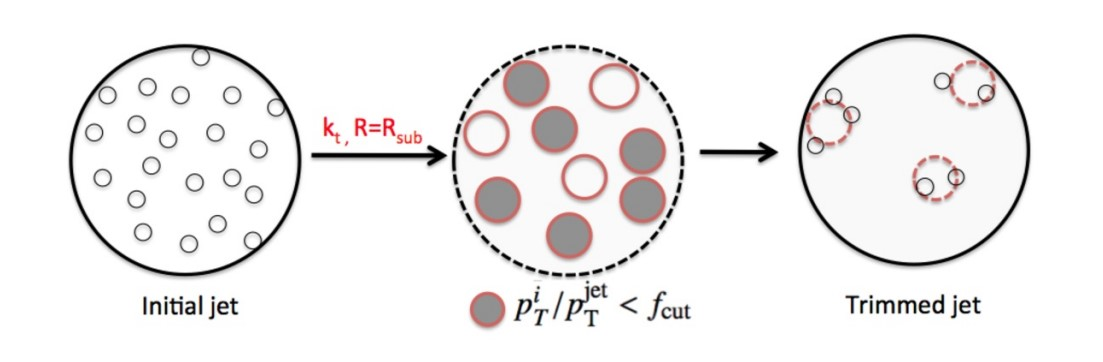
\includegraphics[scale=0.50]{figs/ch4/LR_trim.jpg}
    \caption{ Diagram illustrating the LR jet trimming procedure \cite{LR-jets-opt}.}
\label{fig:trim}
\end{figure}

Mass is then assigned to each trimmed jet according to their four-momentum squared. To improve trimmed jet mass resolution for high-$\textrm{\textit{p}}_{\textrm{T}}$ \gls{lr} jets,
an additional mass ($\textrm{\textit{m}}_{\textrm{TA}}$) is added based on tracks associated with the jet, calculated using Eq. \ref{eq:4.5}. Tracks are associated to sub-jets through a technique called ghost-association. A 
pseudo-particle is reconstructed for each track, having the same coordinates and direction as the track. These pseudo-particles are input into the anti-$\textrm{\textit{k}}_{\textrm{T}}$ algorithm along with 
the energy clusters in the calorimeter. These pseudo-particles are very soft and therefore do not alter the resulting sub-jets. A track is associated to a sub-jet if a corresponding 
pseudo-particle is clustered into the sub-jet. This technique of using ghost-association allows for irregular shaped jets, resulting in an occasional non-cone shaped jet. 

\begin{equation}\label{eq:4.5}
    \textrm{\textit{m}}_{\textrm{TA}} = \frac{\textrm{\textit{p}}_{\textrm{T}}^{\textrm{jet}}}{\textrm{\textit{p}}_{\textrm{T}}^{\textrm{track}}}\textrm{\textit{m}}_{\textrm{track}}
\tag{4.5}
\end{equation}

Where $\textrm{\textit{p}}_{\textrm{T}}^{\textrm{jet}}$ is the transverse momentum of the \gls{lr} jet, $\textrm{\textit{p}}_{\textrm{T}}^{\textrm{track}}$ is the transverse 
momenta of a trimmed anti-$\textrm{\textit{k}}_{\textrm{T}}$ \gls{lr} jet formed from the tracks associated to the jet and $\textrm{m}_{\textrm{track}}$ is the mass of the track jet. The $\textrm{m}_{\textrm{track}}$
is multiplied by this ratio to include energy from the track of the sub-jet. To further improve the jet mass resolution, a combined mass is calculated from a weighted average of the 
two masses as shown in Eq. \ref{eq:4.6}
%
\begin{equation}\label{eq:4.6}
    \textrm{\textit{m}}_{\textrm{comb}} = \textrm{\textit{a}} \cdot \textrm{\textit{m}}_{\textrm{jet}} + \textrm{\textit{b}} \cdot \textrm{\textit{m}}_{\textrm{TA}}
\tag{4.6}
\end{equation}
%
The weights of \textit{a} and \textit{b} must satisfy \textit{a} $+$ \textit{b} = 1 and are derived from resolutions of $\textrm{\textit{m}}_{\textrm{jet}}$ and
$\textrm{\textit{m}}_{\textrm{TA}}$. The final calculated value of $\textrm{\textit{m}}_{\textrm{comb}}$ is the mass of the \gls{lr} jet.
\par
Energy and mass for the trimmed \gls{lr} jets are calibrated in data and simulation to equal values found at particle level in simulated di-jet events \cite{LR-jets-opt}. 
These calibrations are referred to as jet energy scale (\gls{jes}) and jet mass scale (\gls{jms}). The \gls{jes} is corrected first and subsequently the \gls{jms}. In-situ 
calibrations are taken to account for imperfect detector simulations are derived for \gls{jes}, \gls{jer}, and \gls{jms} \cite{LR-jets-cali}. These are performed on all three values of mass from Eq. \ref{eq:4.6}, 
$\textrm{\textit{m}}_{\textrm{jet}}$, $\textrm{\textit{m}}_{\textrm{TA}}$ and $\textrm{\textit{m}}_{\textrm{comb}}$

\subsection{PFlow Object Calibration}

The built PFlow objects are used as input into the anti-$\textrm{\textit{k}}_{\textrm{T}}$ algorithm as discussed in Section \ref{sec:jet-def} \cite{antikt} with \textit{R} = 0.4 to define \gls{sr} jets.
These jets undergo a multi-step calibration. The energy of a reconstructed jet is corrected to match the reconstructed jet at particle level \cite{jes}. This step is known as 
jet energy scale (\gls{jes}). 
\par
Pile-up particles produced in \gls{pp} collisions can deposit energy that may alter the kinematics of the defined \gls{sr} jet. These contributions are subtracted in the 
first step of the \gls{jes} calibration. The energy is compared to di-jet events at particle level from simulation, correcting the four-momentum vectors \cite{jes}.
The next step is referred to as the global sequential calibration (\gls{gsc}). This step corrects dependent parameters such as particles initiating a jet, shower fluctuations, 
and possible showers not detected by the calorimeters or caught in the muon spectrometer. These corrections are evaluated again by using simulated di-jet events.
The final step is to find additional correction factors to mitigate remaining discrepancies to jets from data. The corrections are called in-situ \gls{jes} calibration factors 
and are obtained by evaluating events that contain jets and well calibrated objects, such as electrons, muons or photons. Using momentum balance between these objects, correction 
factors and calculated and applied \cite{jes}. Systematic uncertainties associated with these correction factors arise from modeling in the simulation
\par 
The jet energy resolution (\gls{jer}) is also calibrated. The resolution of an object in the detector depends on background noise of the electronics and energy deposits from 
pile-up. The corrections are found comparing the \gls{jer} from simulated di-jet events to that of data. The correction factors are derived from these di-jet events and 
are applied by smearing the energy distribution to match that of data. Systematic uncertainties are obtained in this calibration step. 

\subsection{Jet Vertex Tagger}

Taggers are tools developed by the \gls{atlas} Flavor Tagging (\gls{ftag}) group to help identify which hadron flavor reconstructed jets originate from. 
The jet vertex tagger (\gls{jvt}) is a tagger used to help identify if tracks are associated to the primary vertex of the hard-scatter \cite{jvt}. There are many \gls{pp} collision that 
occur in a bunch crossing which is the reason for pile-up. So to correctly identify tracks of the collision of interest is crucial. The \gls{jvt} is a multivariate tagger 
algorithm that uses the jet $\textrm{\textit{p}}_{\textrm{T}}$ and its associated tracks. It uses the likelihood of the track being associated to a different collision vertex 
as a discriminating variable. This tagger is only used on jets within $|\textrm{η}| < $ 2.5, for any object that are more forward, a different algorithm is used called the 
forward jet vertex tagger (\gls{fjvt}) \cite{fjvt}.
\par
The \gls{jvt} and \gls{fjvt} efficiencies are measured in data and simulation \cite{jvt,fjvt}. These are determined through simulated events of $\textrm{\textit{Z}} \rightarrow \textrm{a} + \textrm{jets}$,
employing a tag and probe method. Scale factors are derived to correct for discrepancies in the efficiency measurements of data and simulation. 

\section{Heavy-Flavor Tagging}\label{sec:heavyFlavorTagging}

Identifying heavy flavors of quarks plays a crucial role in particle physics analyses. Many interesting physics analyses have b- or c-quarks in their final state. Such as the 
$\textrm{SH} \rightarrow b \bar{b} b \bar{b}$ final state which is discussed in the final part of this thesis.
Flavor tagging (\gls{ftag}) helps discriminate background processes from signal events. Therefore, this process has an important role in not just finding new physics, but also 
precision measurements. 
Since quarks undergo hadronization and cannot exist independently, the quarks themselves cannot be tagged, but rather a color neutral states, b- and c-hadrons. The b-hadrons 
have a lifetime of around 1.5 ps \cite{review-of-hep}, thus decaying after traversing the length of 2.5 mm when it has about 30 GeV. The b-hadron is also associated with a high decay multiplicity of 
an average of five charged particles. Figure \ref{fig:bjet-plots} (a) shows the charged particle decay count from a b-hadron ($\textrm{B}^{\textrm{0}}$), where (b) shows the $\textrm{\textit{p}}_{\textrm{T}}$
fraction the b-hadron carries within the jet which peaks at about 70\%. This results in another important property of a b-jet, it has a high semi-leptonic decay fraction. The typical 
b-jet looks like Figure \ref{fig:bjet-cartoon}. The b-hadron has a decay length L and is indicated by the red dotted line. This leads to a secondary vertex. The decay products from the secondary 
vertex may lead to a tertiary vertex, especially if it's a c-hadron. The displacement of the secondary vertex with respect to the primary vertex is given by a parameter called 
the decay length. The displacement of a track with respect to the primary vertex is parameterized with impact parameters (\gls{ip}s) denoted as $\textrm{d}_{\textrm{0}}$ in 
the figure. This $\textrm{d}_{\textrm{0}}$ \gls{ip} tends to be large for b-hadrons due to the long decay lifetime and large mass (5 GeV). 
\par

\begin{figure}[H]
    \centering
    \subfloat[\centering ]{{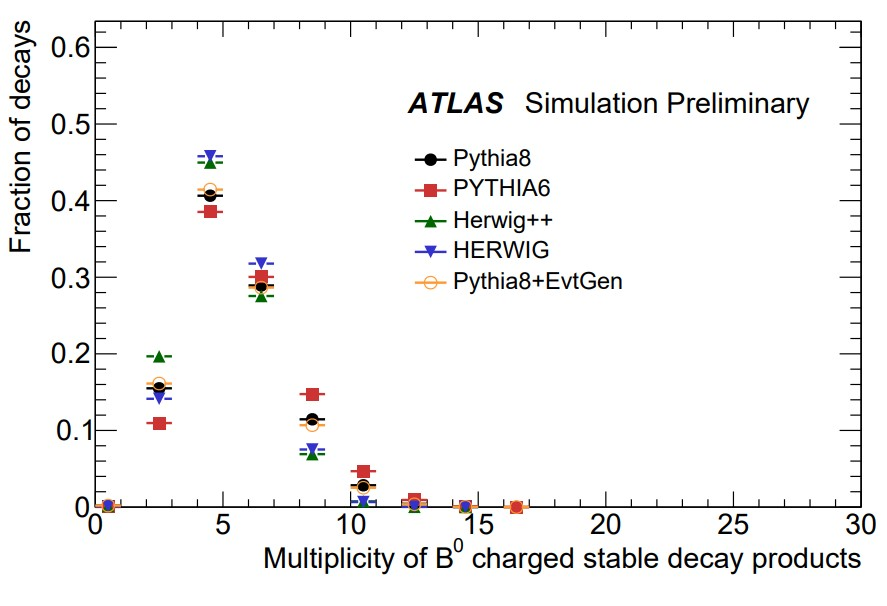
\includegraphics[scale=0.32]{figs/ch4/bjet-stable.jpg}}}%
    \qquad
    \subfloat[\centering ]{{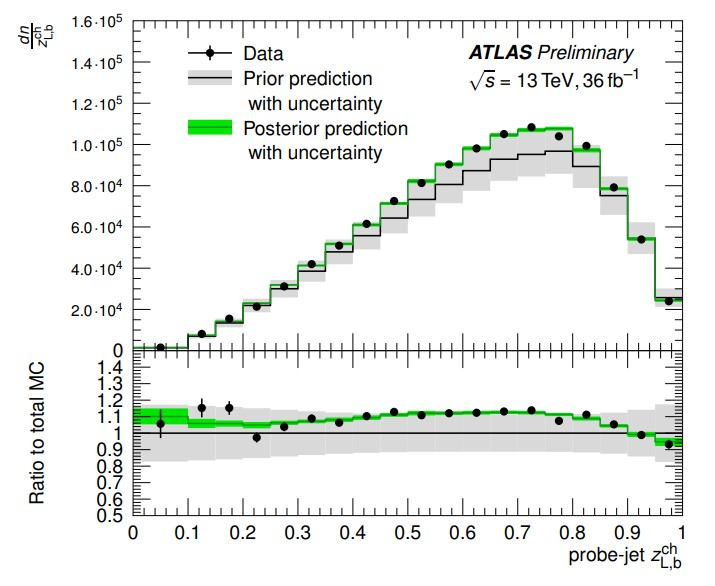
\includegraphics[scale=0.42]{figs/ch4/bjet-pt.jpg}}}%
    \caption{ (a) Decay multiplicity of the b-hadron $\textrm{d}_{\textrm{0}}$ into stable charged products with compared MC generators.
    (b) Fragmentation of b-hadron $\textrm{\textit{p}}_{\textrm{T}}$ }
\label{fig:bjet-plots}
\end{figure}

\begin{figure}[h]
    \centering
    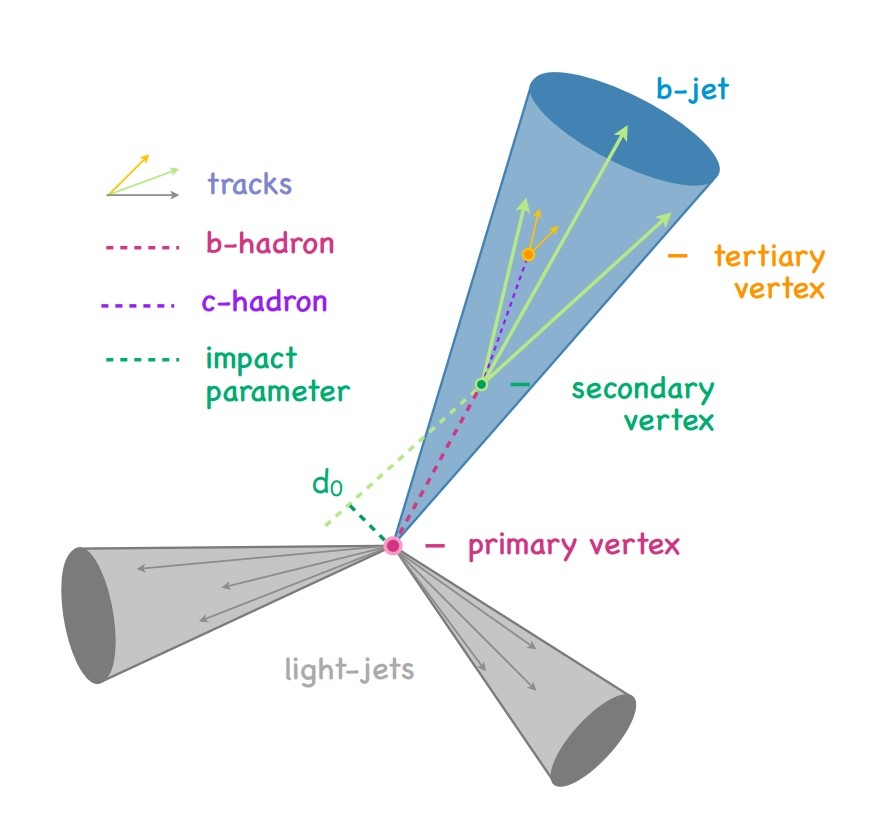
\includegraphics[scale=0.5]{figs/ch4/bjet-cartoon.jpg}
    \caption{ Diagram view of a b-jet with a first, second, and third vertex labeled.}
\label{fig:bjet-cartoon}
\end{figure}

C-hadrons tend to have less stable charged particle multiplicity, shorter decay lengths (resulting in a smaller $\textrm{d}_{\textrm{0}}$) and are lighter. This results in 
similar jet topologies, but not identical. Light-jets originate from lighter quarks which results in tracks being associated with the hadronization itself. These properties 
of c- and light-jets make them separable from b-jets. All these unique b-jet properties are targeted by \gls{ftag} tools developed to \textit{tag} a b-hadron. There are several 
b-tagging algorithms, all attempting to extract specific features of the b-hadron's information. These baseline algorithms can be categorized into three categories:
the \gls{ip} based algorithms called Impact parameter 2(3) Dimensional (\gls{ip2d}, \gls{ip3d}), Recurrent Neural Network \gls{ip} (\gls{rnnip}) and Deep Impact Parameters (\gls{dips});
the vertex-based algorithms of Secondary Vertex (\gls{sv1}) and JetFitter; lastly the soft-muon tagger (\gls{smt}).
\par
These baseline taggers are then combined \textit{high-level taggers} such as a multivariate boosted-decision tree (\gls{mv2}), deep-learning based DL1 (\gls{dl1}), and a graph 
neural network (\gls{nn}) tagger (\gls{gn1}). \gls{dl1} is studied for the \gls{hllhc} in chapter \ref{ch5} and the following sections will describe its related baseline taggers.
Figure \ref{fig:ftag-diagram} is a diagram showing the baseline input for each of the high-level taggers. 

\begin{figure}[h]
    \centering
    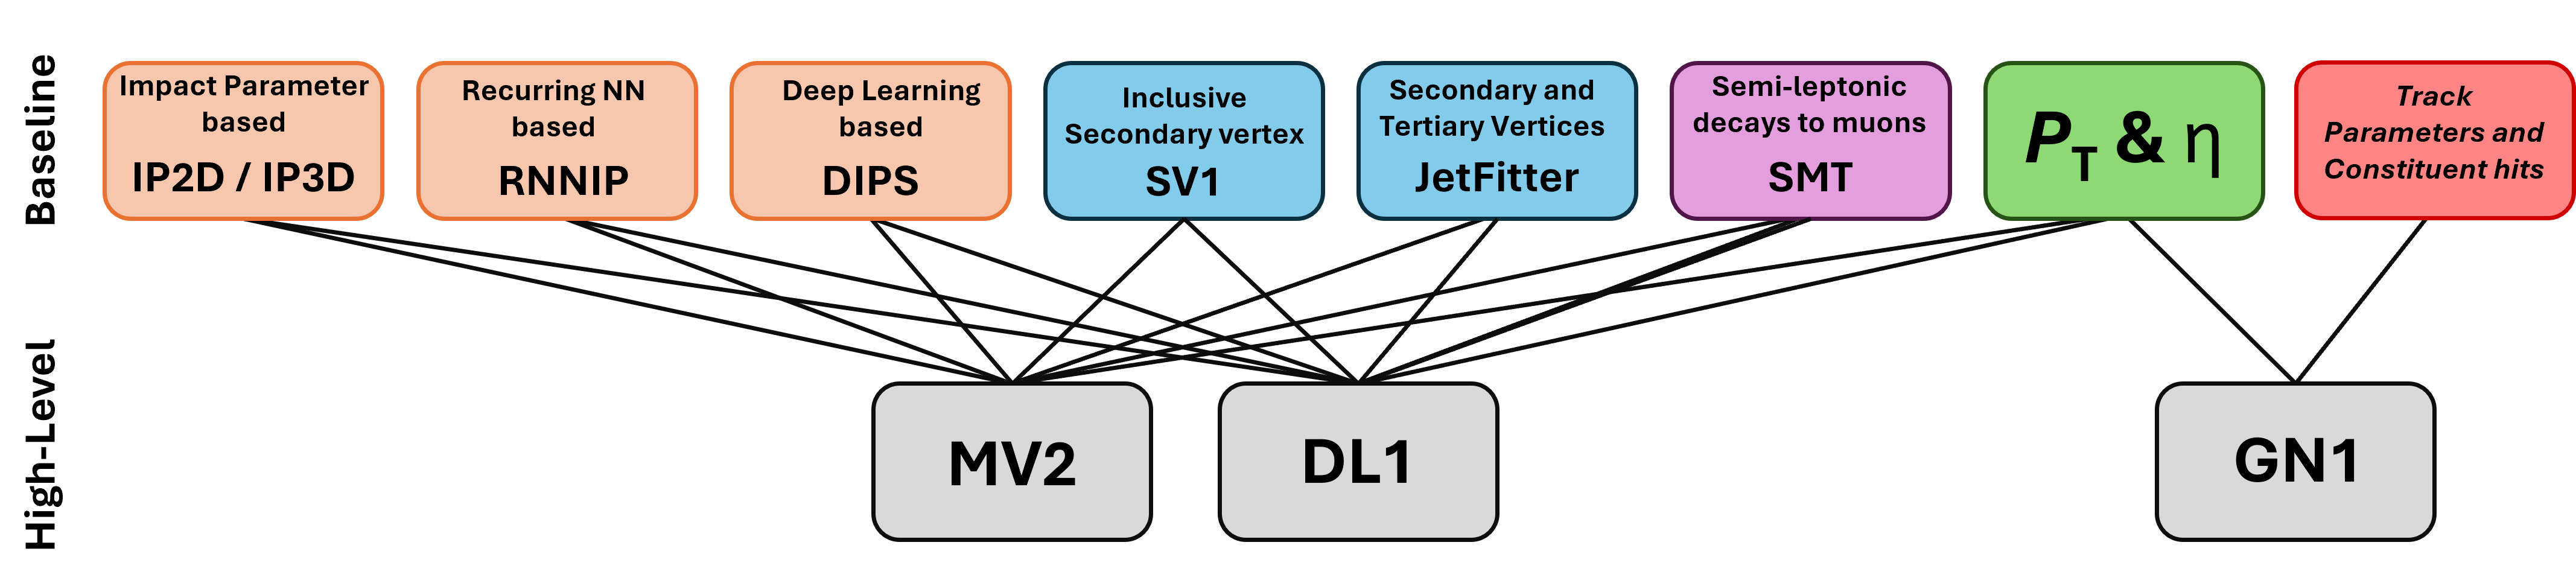
\includegraphics[scale=0.5]{figs/ch4/ftag-diagram.png}
    \caption{ Diagram of FTAG baseline and high-level taggers.}
\label{fig:ftag-diagram}
\end{figure}

\subsection{Impact Parameter Algorithms}\label{sec:ip-algo}

A b-hadron has the longest lifetime of any quarks which results in a long decay length and a displaced secondary vertex. The \gls{ip} is the point of closest approach of 
tracks from the b-hadron decay to the primary vertex. This parameter can be split into two parts, the $\textrm{d}_{\textrm{0}}$ as seen in Figure \ref{fig:bjet-cartoon}, and 
a longitudinal part $\textrm{\textit{z}}_{\textrm{0}} \textrm{sin}{\theta}$. A variable of the \gls{ip} is the signed lifetime significances $\textrm{s}_{\textrm{d}_{\textrm{0}}}$ 
= $\frac{\textrm{d}_{\textrm{0}}}{\sigma_{\textrm{d}_{\textrm{0}}}}$ and $\textrm{s}_{\textrm{\textit{z}}_{\textrm{0}}}$ = $ \frac{\textrm{\textit{z}}_{\textrm{0}} \textrm{sin}{\theta}}{\sigma_{\textrm{\textit{z}}_{\textrm{0}} \textrm{sin}{\theta}}}$.
are calculated corresponding to the \gls{ip} divided by its uncertainty, as shown in Figure \ref{fig:ip-sig}. The sign of this variable is assigned by extrapolating the track back to the 
primary vertex. This value is negative if the jet axis has to be extended backwards from the primary vertex to cross the track or its projection, otherwise it's positive. 
The \gls{ip} algorithms are used to satisfy certain criteria such as: $\textrm{\textit{}}_{\textrm{T}}^{\textrm{track}} >$ 1 GeV, the \gls{ip}s have to fulfill  $|\textrm{d}_{\textrm{0}}| < $ 
1 mm, and $|\textrm{\textit{z}}_{\textrm{0}} \textrm{sin}{\theta}| <$ 1.5 mm. Additional requirements are required for the number of hits in the silicon layers: $\textrm{N}_{\textrm{hits}}^{\textrm{Si}}
\geq$ 7 as well as an upper limit of silicon and pixel layer holes  $\textrm{N}_{\textrm{holes}}^{\textrm{Si}} \leq$ 2 and  $\textrm{N}_{\textrm{holes}}^{\textrm{pixel}} \leq$ 1.
The following sections briefly describes the IPxD baseline taggers and the \gls{dips} tagger. The \gls{rnnip} tagger will not be described as it is outside the scope of this thesis.
\begin{figure}[H]
    \centering
    \subfloat[\centering ]{{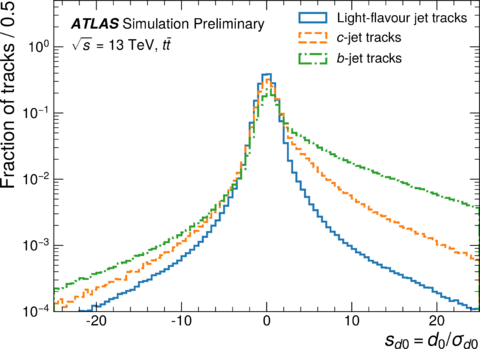
\includegraphics[scale=0.45]{figs/ch4/signed_d0.png}}}%
    \qquad
    \subfloat[\centering ]{{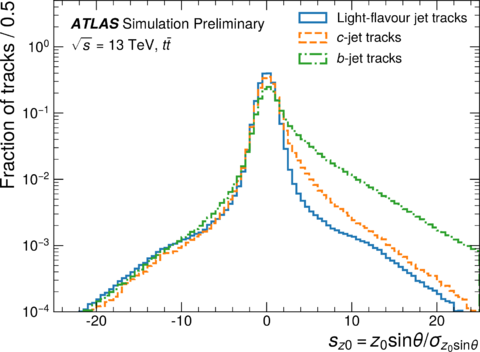
\includegraphics[scale=0.45]{figs/ch4/signed_z0.png}}}%
    \caption{ The signed IP significances variable shown for b-, c-, and light-jets for (a) transverse and (b) longitudinal components in $t\bar{t}$ events }
\label{fig:ip-sig}
\end{figure}

\subsubsection{IPxD}

The IPxD taggers comprise of two algorithms: the \gls{ip2d} which only uses the transverse \gls{ip} $\textrm{d}_{\textrm{0}}$ variable which tends to be less sensitive to pile-up, and 
the \gls{ip3d} tagger which uses both the transverse $\textrm{d}_{\textrm{0}}$ and $\textrm{\textit{z}}_{\textrm{0}} \textrm{sin}{\theta}$ variables \cite{btag-opt-2016}. The track categorization is based on 
pixel layer hit patterns as pre-defined by reference templates for b, c, and light hadrons. The final discriminant is a Log-Likelihood ratio (\gls{llr}) of probabilities of 
being any of the three hadrons. This \gls{llr} is described by Eq.~\ref{eq:4.7}.

\begin{equation}\label{eq:4.7}
    \textrm{IPxD}_{\textrm{l,c,cl}} = \sum_{\textrm{i}\in \textrm{tracks}} \textrm{log}\left(\frac{\textrm{P}^{\textrm{i}}_{\textrm{b,b,c}}}{\textrm{P}^{\textrm{i}}_{\textrm{l,c,l}}}\right)
\tag{4.7}
\end{equation}

The probability density functions to calculate $\textrm{P}_{\textrm{b}}$, $\textrm{P}_{\textrm{c}}$ and $\textrm{P}_{\textrm{l}}$ are extracted from \gls{mc} simulations.
Table \ref{tab:ipxd-variables} shows the six different variables for the IPxD tagger used to tag jets. The IPxD baseline taggers are used as input into the high-level taggers such as 
MV2 and DL1.

\begin{table}[t]
    \centering 
    \begin{tabular}{ |m{4em} |m{6cm} |}
        \hline
        \multicolumn{2}{|c |}{IPxD Discriminating Variables}\\
        \hline\hline
        Variable & Description \\
        \hline
         & LLR based on signed significance \\
         $\textrm{IPxD}_{\textrm{l}}$ & b- from light flavor jets \\
         $\textrm{IPxD}_{\textrm{c}}$ & b- from c-jets \\
         $\textrm{IPxD}_{\textrm{cl}}$ & c- from light flavor jets \\
         \hline
    \end{tabular}
    \caption{Variables for the IP2D and IP3D taggers (3 each)}
    \label{tab:ipxd-variables}
\end{table}

\subsubsection{DIPS}\label{sec:dips}

The \gls{dips} is a machine-learned algorithm that uses the \gls{ip} variables as input for a Deep Sets architecture \cite{Deep_sets}, treating the elements as a set without any specific order. 
The formalism of \gls{dips} has $\textit{\textrm{p}}_{\textit{\textrm{i}}}$ which is the vector representation of the inputs associated with the $\textit{\textrm{i}}^{\textit{\textrm{th}}}$ 
track in the jet, then the Deep Sets architecture applies its weight $\phi$ to each track. Tracks are then summed over and has additional processing in the form of a feed forward 
\gls{nn} (\textit{F}) as described in Eq. \ref{eq:4.8}.
%
\begin{equation}\label{eq:4.8}
    \mathcal{O}({\textit{\textrm{p}}_{\textrm{1}},...,\textit{\textrm{p}}_{\textit{\textrm{n}}}}) = \textrm{\textit{F}}\left(\sum^{\textrm{n}}_{\textit{\textrm{i}}=\textrm{1}}\phi (\textrm{\textit{p}}_{\textit{\textrm{i}}})\right)
\tag{4.8}
\end{equation}
%
where $\mathcal{O}({\textit{\textrm{p}}_{\textrm{1}},...,\textit{\textrm{p}}_{\textit{\textrm{n}}}})$ represents the b-, c-, and light- class probabilities. The architecture 
bisects the problem into operations over the inputs and over the sets. The track network $\phi$ extracts the relevant track information and the forwarding jet-network \textit{F} 
accounts for the correlations between the tracks \cite{DIPS}. Permutation invariance of the set is encoded using the sum operation. Since \gls{dips} encodes this permutation 
invariance, a much more natural representation of the data is made, allowing the machine learning (\gls{ml}) algorithm to be trained more effectively. This algorithm outperforms 
IPxD and \gls{rnnip} algorithms. 
\par
The \gls{ml} model of \gls{dips} outputs class probabilities of b-, c- and light-jets ($\textit{\textrm{p}}_{\textit{\textrm{b}}}, \textit{\textrm{p}}_{\textit{\textrm{c}}}, \textit{\textrm{p}}_{\textit{\textrm{l}}}$).
A discriminant is made from a combination of these three probabilities dictating whether a jet is b-tagged or not, this discriminant is given by Eq. \ref{eq:4.9}.
%
\begin{equation}\label{eq:4.9}
    \textit{\textrm{D}}_{\textit{\textrm{b}}} = \textrm{log} \frac{\textit{\textrm{p}}_{\textit{\textrm{b}}}}{(\textrm{1}-\textit{\textrm{f}}_{\textit{\textrm{c}}})\textit{\textrm{p}}_{\textit{\textrm{l}}}+\textit{\textrm{f}}_{\textit{\textrm{c}}}\textit{\textrm{p}}_{\textit{\textrm{c}}}}
\tag{4.9}
\end{equation}
%
where $\textit{\textrm{f}}_{\textit{\textrm{c}}}$ is a free parameter that helps balance the rejection rate between light-jets and c-jets for a given b-tagging efficiency. This 
is optimized post-training. A few input variables for \gls{dips} are scaled and shifted due to a mean that is not close to zero, this process is described in reference \cite{DIPS}. 
A list of \gls{dips} input features can be seen in Table \ref{tab:dips-variables}. The features that required additional preprocessing are noted.

\begin{table}[ht]
    \centering 
    \begin{tabular}{ |m{8em} |m{10cm} |m{5em} |}
        \hline
        \multicolumn{3}{|c |}{DIPS Input Features}\\
        \hline\hline
        Input & Description & Preprocessed\\
        \hline
         $\textrm{s}_{\textrm{d}_{\textrm{0}}}$ & $\textrm{d}_{\textrm{0}}$/$\sigma_{\textrm{d0}}$: Transverse IP significance &  \\
         $\textrm{s}_{\textrm{z}_{\textrm{0}}}$ & $\textrm{\textit{z}}_{\textrm{0}}\textrm{sin}\theta$/$\sigma_{\textrm{\textit{z}}\textrm{0sin}\theta}$: Longitudinal IP significance & \\
         $\textrm{log}\textrm{\textit{p}}_{\textrm{T}}^{\textrm{frac}}$ & $\textrm{log}\textrm{\textit{p}}_{\textrm{T}}^{\textrm{frac}}$ /$\textrm{\textit{p}}_{\textrm{T}}^{\textrm{jet}}$: Logarithm of fraction of the jet $\textrm{\textit{p}}_{\textrm{T}}$ & \checkmark \\
          & carried by the track &  \\
         $\textrm{log}∆\textrm{R}$ & Logarithm of opening angle between the track & \checkmark \\
          & and the jet axis & \\
         IBL hits & Number of hits in the IBL: could be 0, 1, or 2& \\
         PIX1 hits & Number of hits in the next-to-innermost pixel layer: could be 0, 1. or 2& \\
         shared IBL hits & shared IBL hits & \\
         split IBL hits & Number of split hits in the IBL& \checkmark \\
         nPixHits & Combined number of hits in the pixel layers& \\
         shared pixel hits & Number of shared hits in the pixel layers & \\
         split pixel hits & Number of split hits in the pixel layers& \\
         nSCTHits & Combined number of hits in the SCT layers& \checkmark \\
         shared SCT hits & Number of shared hits in the SCT layers& \\
         \hline
    \end{tabular}
    \caption{Input variables for DIPS}
    \label{tab:dips-variables}
\end{table}



\subsection{Secondary Vertex Algorithm}

The secondary vertex \gls{sv1} algorithm reconstructs a single displaced vertex in a jet using tracks. Due to hardware constraints, sometimes the track resolution in the \gls{id}
is not always able to resolve the entire decay cascade of a hadron in every jet. Therefore the criteria of reconstruction is only a single vertex, which is a good approximation
for a b-jet. The first step matches all two-track vertices, rejecting vertices that are compatible with tracks associated with long-lived particles, photon conversions or hadronic 
interactions with detector material. The next step is combine each accepted two-tracks into secondary vertices while removing all rejected tracks. Important information can 
be extracted from \gls{sv1} such as the vertex mass, decay length and its significance, number of associated tracks as well as the $∆\textrm{R}$ between the jet and the 
secondary vertex. Table \ref{tab:sv1} shows an overview of the variables for \gls{sv1}.

\begin{table}[ht]
    \centering 
    \begin{tabular}{ |m{5em} |m{14cm} |}
        \hline
        \multicolumn{2}{|c |}{SV1 Variables}\\
        \hline\hline
        Variable & Description \\
        \hline
         $\textrm{N}^{\textrm{SV1}}_{\textrm{trkAtVtx}}$ & Number of tracks associated to the SV \\
         $\textrm{N}^{\textrm{SV1}}_{\textrm{2trkAtVtx}}$ & Number of reconstructed two-track vertices candidates within the jet \\
         $\textrm{m}^{\textrm{SV1}}_{\textrm{inv}}$ & Invariant mass of the SV calculated from the associated tracks\\
         $\textrm{f}^{\textrm{SV1}}_{\textrm{E}}$   & Energy fraction of the SV associated tracks with respect to all tracks of the jet\\
         $∆\textrm{R}(\textrm{jet, SV})$    & $∆\textrm{R}$ between the jet axis and the secondary vertex relative to the primary vertex\\
         $\textrm{L}^{\textrm{SV1}}_{\textrm{xy}}$  & Reconstructed SV transverse decay length \\
         $\textrm{L}^{\textrm{SV1}}_{\textrm{xyz}}$ & Reconstructed SV decay Length \\
         $\textrm{S}^{\textrm{SV1}}_{\textrm{xyz}}$ & Decay Length significance \\
         \hline
    \end{tabular}\hfill
    \caption{ Variable overview for the SV1 algorithm \cite{btag-opt-2016}}
    \label{tab:sv1}
\end{table}

\subsection{JetFitter}

The decay chain multi-vertex reconstruction algorithm, a.k.a. JetFitter, is the second displaced vertex finder algorithm behind \gls{sv1} \cite{btag-opt-2016}. This algorithm 
aims to reconstruct the decay cascade topology of weakly decaying b- and c- hadrons. It assumes the primary, secondary, and the tertiary vertices are aligned in one line in the 
direction of the hadron's trajectory. The goal of this assumption is to cope with the finite track resolution. After an initial track selection of removing tracks associated to 
the primary vertex using a Kalman Filter \cite{kalman}. The resulting variables of JetFitter are shown in Table \ref{tab:jf-btag}. 
\par
This algorithm allows for special variables for the c-hadron exploiting the fact that the JetFitter vertex would be close to the primary vertex. These are chosen to differentiate 
the topologies between the b- and c- hadron. C-hadrons have lower decay multiplicity than the b-hadron due to their lower mass, thus decay products carry a larger momentum 
percentage along with a larger rapidity with respect to the jet axis. These variables are shown in Table \ref{tab:jf-ctag}.

\begin{table}[ht]
    \centering 
    \begin{tabular}{ |m{6em} |m{12cm} |}
        \hline
        \multicolumn{2}{|c |}{JetFitter Variables}\\
        \hline\hline
        Variable & Description \\
        \hline
         $\textrm{m}^{\textrm{JF}}_{\textrm{inv}}$ & Invariant mass of tracks associated to one or more displaced vertices \\
         $\textrm{f}^{\textrm{JF}}_{\textrm{E}}$ & Charged jet energy fraction in the secondary vertex \\
         $\textrm{S}^{\textrm{JF}}_{\textrm{xyz}}$ & Decay length significance of the displaced vertex\\
         $\textrm{N}^{\textrm{JF}}_{\textrm{1-trk vertices}}$   & Number of 1-track displaced vertices\\
         $\textrm{N}^{\textrm{JF}}_{\leq \textrm{2-trk vertices}}$ & Number of vertices with more than one track\\
         $∆\textrm{R}^{\textrm{JF}} (\textrm{P}_{\textrm{jet}}, \textrm{P}_{\textrm{vtx}})$     & $∆\textrm{R}$  between jet axis and the vectorial sum of all track momenta\\
         $\textrm{N}^{\textrm{JF}}_{\textrm{trks}}$  & Number of tracks associated to SV \\
         $\textrm{N}^{\textrm{JF}}_{\textrm{vertices}}$ & Number of reconstructed vertices \\
         \hline
    \end{tabular}\hfill
    \caption{ Variable overview of JetFitter algorithm for b-tagging \cite{btag-opt-2016}}
    \label{tab:jf-btag}
\end{table}

\begin{table}[H]
    \centering 
    \begin{tabular}{ |m{7em} |m{10cm} |}
        \hline
        \multicolumn{2}{|c |}{JetFitter C-Hadron Variables}\\
        \hline\hline
        Variable & Description \\
        \hline
         $\textrm{L}^{\textrm{\textrm{JF}}}_{\textrm{xyz}}$ & Displacement of SV from the primary vertex \\
         $\textrm{L}^{\textrm{\textrm{JF}}}_{\textrm{xy}}$ &  Transverse displacement of SV from the primary vertex\\
         $\textrm{min}(\textrm{Y}^{\textrm{JF}}_{\textrm{trk}})$ & Minimal rapidity of tracks within the jet \\
         $\textrm{max}(\textrm{Y}^{\textrm{JF}}_{\textrm{trk}})$ & Maximum rapidity of tracks within the jet \\
         $\textrm{avg}(\textrm{Y}^{\textrm{JF}}_{\textrm{trk}})$ & Average rapidity of tracks within the jet\\
         $\textrm{min}(\textrm{Y}^{\textrm{JF}}_{\textrm{trk, SV}})$ & Minimal rapidity of SV tracks\\
         $\textrm{max}(\textrm{Y}^{\textrm{JF}}_{\textrm{trk, SV}})$ & Maximum rapidity of SV tracks\\
         $\textrm{avg}(\textrm{Y}^{\textrm{JF}}_{\textrm{trk, SV}})$ & Average rapidity of SV tracks\\
         $\textrm{m}^{\textrm{JF}}_{\textrm{inv}} $ & Invariant mass of tracks associated to the SV\\
         $∆\textrm{E}^{\textrm{JF}}$     & Energy of tracks associated to SV\\
         $\textrm{f}^{\textrm{JF}}_{\textrm{E}}$  & Charged jet energy fraction of SV \\
         $\textrm{N}^{\textrm{JF}}_{\textrm{trks}}$ & Number of tracks associated to the SV \\
         \hline
    \end{tabular}\hfill
    \caption{ Variable overview of JetFitter algorithm for c-tagging \cite{btag-opt-2016}}
    \label{tab:jf-ctag}
\end{table}

\section{High-Level Taggers}

Baseline taggers are optimized for single properties of b-hadron decays. High-level taggers are multivariate taggers comprised of the baseline taggers previously described 
and as seen in Figure \ref{fig:ftag-diagram}. There are three high-level taggers that are currently deployed in ATLAS: the boosted decision tree (\gls{bdt}) based tagger MV2, 
the deep learning based DL1 and the graph \gls{nn} GN1. Currently, DL1 is the standard tagger within \gls{atlas}, but GNN based taggers have proven to be more effective and are currently being developed to replace it. DL1 is 
explored in higher detail in chapter \ref{ch5}. 

\subsection{Working Points}

As briefly discussed in Section \ref{sec:muon-reco}, \gls{wp}s are deployed for the high-level taggers to cover various needs in physics analyses. These \gls{wp}s are defined using 
the b-tagging efficiency on $t\bar{t}$ \gls{mc} samples. These single cut \gls{wp}s are used since having a full continuous b-tagging discriminant would require a continuous 
calibration in extremely fine efficiency bins. This task would take enormous time and require immense complexity. The tagging efficiency is described in Eq. \ref{eq:4.10}
%
\begin{equation}\label{eq:4.10}
    \varepsilon^{\textrm{j}} = \frac{\textrm{N}^{\textrm{j}}_{\textrm{pass}}(\mathcal{D} > \textrm{T}_\textrm{f})}{\textrm{N}^{\textrm{j}}_{\textrm{total}}} 
\tag{4.10}
\end{equation}
%
where $\textrm{N}^{\textrm{j}}_{\textrm{pass}}(\mathcal{D} > \textrm{T}_\textrm{f})$ are the number of jets of flavor \textit{j} passed the cut $\textrm{T}_{\textrm{f}}$ on the tagger 
discriminant $\mathcal{D}$ and $\textrm{N}^{\textrm{j}}_{\textrm{total}}$ are all jets of flavor j before the cut. The \gls{wp}s are defined based on b-jet efficiency $\varepsilon^{\textrm{j}}$
evaluated on $t\bar{t}$ \gls{mc} samples. In \gls{atlas} there are four \gls{wp}s defined as seen in Table \ref{tab:bjet-eff}. The inverse of each \gls{wp} characterizes the c- and light- jet rejection rate.
Misidentification improves with lower signal efficiency, therefore rejecting more background, trading off lower signal statistics. Within a physics analysis, every jet that passes a 
\gls{wp} is considered a b-jet. Each high-level tagger that is described in the following sections have different rates of b-tagging efficiencies, meaning the number of tagged 
b-jets in an analysis will depend on which tagger is used. Therefore high tagging efficiencies are sought after, encouraging physicists to use the latest technological advances.
The \gls{bdt} based MV2 was the standard tagger until Deep Sets architectures overtook and shown to be much more efficient, thus DL1 has now become the new standard. 
Recent developments in the past year has shown that graph \gls{nn}s can exploit track information much more profoundly, resulting in much higher tagging efficiencies than 
the DL1 tagger and is expected to take its place.

\begin{table}[ht]
    \centering 
    \begin{tabular}{ |m{6em} |m{4cm} |}
        \hline
        \multicolumn{2}{|c |}{Working Points for B-Tagging in ATLAS}\\
        \hline\hline
        Cut & b-tagging efficiency \\
        \hline
        loose & 85\% \\
        medium & 77\% \\
        tight & 70\% \\
        very tight & 60\% \\
        \hline
    \end{tabular}\hfill
    \caption{ Summary of b-tagging single cut WPs}
    \label{tab:bjet-eff}
\end{table}


\subsection{MV2}

The high-level tagger MV2 used to be the recommended tagger for EMTopo jets for Run 2 of ATLAS. This tagger used 24 inputs from the baseline taggers as input for the \gls{bdt}
training as well as $\textrm{\textit{p}}_{\textrm{T}}$ and $|\textrm{η}|$. Training the MV2 tagger used what is called a \textit{hybrid} sample which is a mixture of $t\bar{t}$ and Z' 
events. This is to ensure there is a large coverage of the $\textrm{\textit{p}}_{\textrm{T}}$ spectrum. The \gls{bdt} used b-jets as the signal class and c- and light- jets as a background class.
To balance the performance between the c-jet and light-jet rejection, a c-jet fraction $\textrm{f}_{\textrm{c}}$ was set to 7\% and therefore a light jet fraction of 93\%. The end result 
was named MV2c10. Figure \ref{fig:mv2_eff} shows the performance of the MV2, DL1 and baseline taggers in terms of background rejection as a function of b-tagging efficiency.

\begin{figure}[H]
    \centering
    \subfloat[\centering ]{{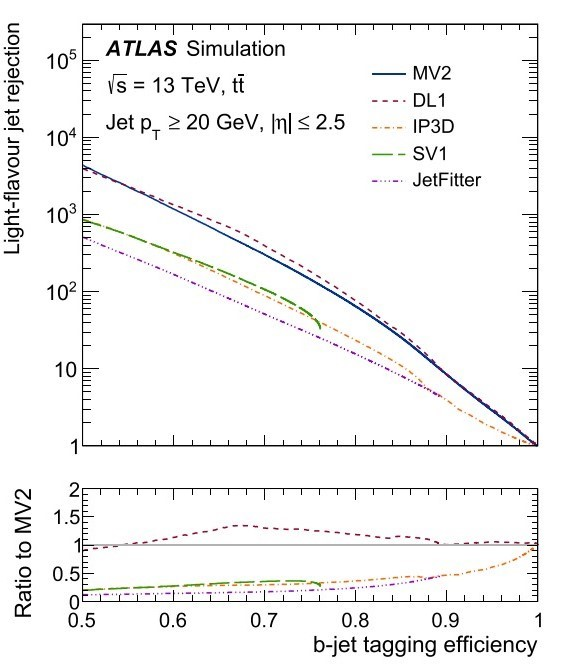
\includegraphics[scale=0.5]{figs/ch4/mv2_effu.jpg}}}%
    \qquad
    \subfloat[\centering ]{{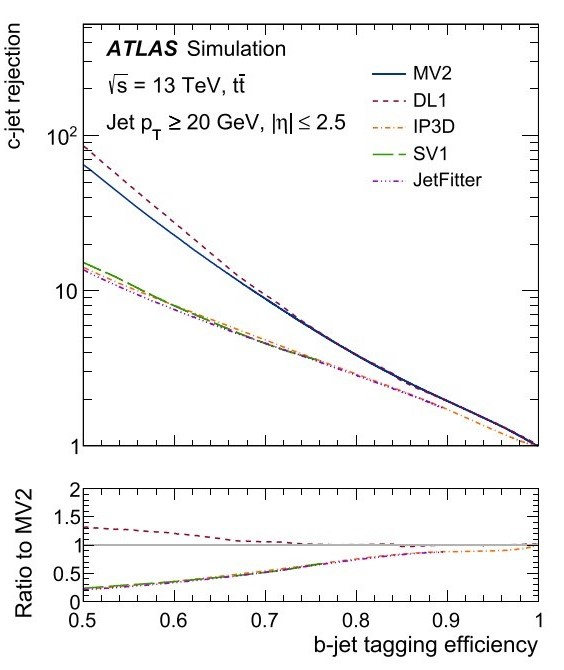
\includegraphics[scale=0.5]{figs/ch4/mv2_effb.jpg}}}%
    \caption{ The (a) light-jet and (b) c-jet rejections versus the b-jet tagging efficiency for the baseline taggers IP3D, SV1, JetFitter and the high level taggers MV2 and DL1. Evaluated on $t\bar{t}$ MC events \cite{btag-iden-eff}}
\label{fig:mv2_eff}
\end{figure}

\subsection{DL1}\label{sec:DL1-ch4}

The high-level DL1 tagger is a deep feed-forward \gls{nn} with three output nodes that correspond to the b-, c-, and light- flavor jet probabilities. The ReLU activation function is used 
for each layer while the last layer uses the softmax activation function. Using the softmax function for the output layer allows the output to be interpreted as probabilities. 
The final b-tagging log-likelihood discriminant score is calculated from the multi-class output using Eq. \ref{eq:4.11}.
%
\begin{equation}\label{eq:4.11}
    \mathcal{D}_{\textrm{b}}(\textrm{f}_{\textrm{c}}) = \textrm{log}\left(\frac{\textrm{p}_{\textrm{b}}}{\textrm{f}_{\textrm{c}} \cdot \textrm{p}_{\textrm{c}} + (\textrm{1}-\textrm{f}_{\textrm{c}}) \cdot \textrm{p}_{\textrm{l}} }\right)
\tag{4.11}
\end{equation}
%
where $\textrm{p}_{\textrm{b}}$, $\textrm{p}_{\textrm{c}}$ and $\textrm{p}_{\textrm{l}}$ are the output scores of DL1 representing the probabilities for the jet to be a b-jet, c-jet 
or a light-jet, respectively. The c-jet fraction $\textrm{f}_{\textrm{c}}$ allows tuning to balance the performance of the c-jet and light-jet rejection. The c-jet rejection increases 
as a function of $\textrm{f}_{\textrm{c}}$ and light-flavor decreases as a function of $\textrm{f}_{\textrm{c}}$. An advantage of using the DL1 compared to MV2 is that the 
discriminant can be rewritten to perform c-jet tagging with b-jet rejection. This new rewritten discriminant can be seen in Eq.~\ref{eq:4.12}
%
\begin{equation}\label{eq:4.12}
    \mathcal{D}_{\textrm{c}}(\textrm{f}_{\textrm{b}}) = \textrm{log}\left(\frac{\textrm{p}_{\textrm{c}}}{\textrm{f}_{\textrm{b}} \cdot \textrm{p}_{\textrm{b}} + (\textrm{1}-\textrm{f}_{\textrm{b}}) \cdot \textrm{p}_{\textrm{l}} }\right)
\tag{4.12}
\end{equation}
%
where  $\textrm{f}_{\textrm{b}}$ is a floating value for the b-jet fraction. DL1 has shown many positives over MV2. The tagger is effectively maintained with much less person power,
while also fewer variables have to be calculated and stored, saving computing power. The DL1 tagger is a family of high-level multivariate taggers. These taggers differ from the 
baseline tagger inputs, they are as follows: baseline DL1, DL1r, DL1rmu, and DL1d. The DL1 baseline uses the same variables as MV2 with the additional JetFitter variables for c-jet 
identification. DL1r configuration uses the \gls{rnnip} instead of the baseline IPxD taggers. The DL1rmu exploits the soft-muon information. Lastly, the DL1d uses the baseline taggers 
SV1, JetFitter but uses the \gls{dips} instead of the baseline IPxD. More information is given on the DL1d tagger in Chapter \ref{ch5}.


\subsection{GN1}\label{sec:gn1}

The GN1 tagger is currently the latest and greatest particle identification algorithm. It differs from the previously described high-level taggers in a few ways. GN1 does not make 
use of the underlying baseline taggers but instead exploits the internal structure of the jet through the use of two auxiliary training objectives: the grouping of tracks originating 
from a common vertex, and the prediction of the underlying physics processes \cite{gnn-ftag}. The graph neural network takes 2 kinematic and 21 track variables as training input. Using auxiliary 
tasks removes the need to add the baseline taggers, therefore simplifying the training process and allowing the tagger to be more versatile in training phase space. The algorithm 
is trained on \textit{truth-information} obtained through simulations. 
\par
The GN1 combines a graph neural network architecture with auxiliary training objectives. Initially, the two jet inputs (transverse momentum and signed pseudorapidity) are fed 
into a per-track initialization network with three hidden layers, each containing 64 neurons. These three layers are a Deep Sets architecture such as the technique used by DL1.
A fully connected graph is built from the outputs of these three Deep Set layers. Each node $\textrm{\textit{h}}_{\textrm{i}}$ in the graph represents a single track in the jet, 
characterizing a feature vector. The output nodes from the Deep Set architecture are used to populate the graph. Outputs from each graph layer are aggregated features of each node 
$\textrm{\textit{h}}_{\textrm{i}}$ and neighboring nodes $\textrm{\textit{N}}_{\textrm{i}}$. The feature vectors of each node are fed into a fully connected \gls{nn} layer that 
produces updated values of the vector. These updated features are used to compute edge scores of each node (scores calculated from neighboring nodes). A non-linear activation 
function is used while a softmax function calculates weights for each pair of nodes using the edge scores. Finally, an updated node representation is computed by taking the 
weighted sum over each updated node representation. After the graph network is implemented, these outputs are used in a node classification network to predict track truth origin. 
A diagram of the entire network architecture is seen in Figure \ref{fig:gnn-diagram}. The track and jet kinematic input variables for the \gls{gn1} tagger are listed in Table~\ref{tab:gn1-var} within the Appendix \ref{appendix:gn1-upgrade}. The next version of \gls{gn1} is called GN2 and is currently expected to replace its predecessor. 

\begin{figure}[h]
    \centering
    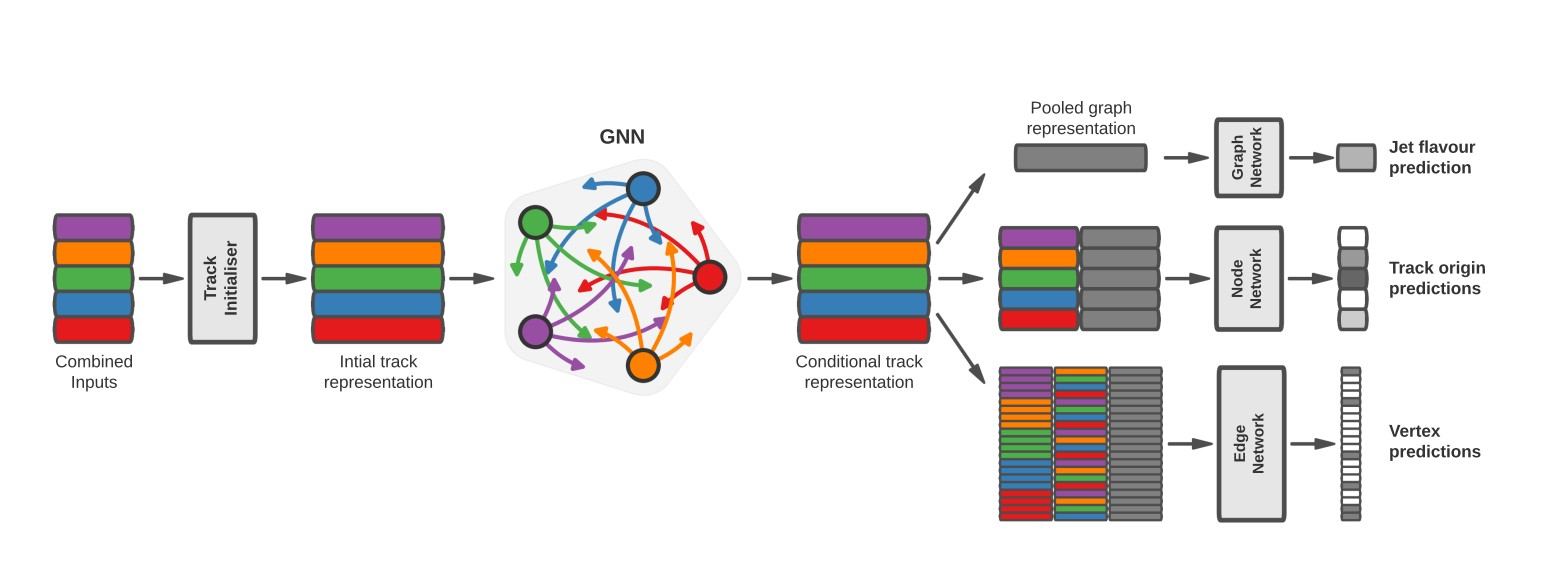
\includegraphics[scale=0.38]{figs/ch4/GNN-diagram.jpg}
    \caption{ The network diagram of GN1. First, a Deep Sets architecture is used to populate node features in a GNN. The GNN outputs are used to predict jet flavor, track origins, and track-pair vertex compatibility. \cite{gnn-ftag}}
\label{fig:gnn-diagram}
\end{figure}



\section{Event Simulation}\label{sec:event-sim}

Simulated \gls{pp} events are used in every physics analysis while also being vital in event reconstruction calibrations. They also play an important role in simulating \gls{bsm} 
models which are used to help define new phases spaces for the chance of detecting new physics. Simulated events are used later in this thesis as \gls{ml} input and are vital 
in deploying efficient particle identification algorithms. \gls{bsm} simulations are also used in the Anomaly Detection analysis in Chapter~\ref{ch6} to show separation 
between standard \gls{sm} events and the anomalous \gls{bsm} events. 
\par
Event simulations not only simulate kinematics of particles within the \gls{sm} (or beyond of it) but are also used to show how simulated particles would interact with the 
\gls{atlas} detector. Due to the complexity of integral emerging from \gls{qft} calculations, Monte Carlo \gls{mc} techniques are used in the simulations \cite{workman}.

\subsection{Monte Carlo Generators}


Every event generation is typically divided into two parts: the matrix element generation that describes the hard scatter and secondly the parton showering and hadronization modeling 
which includes the initial state radiation (\gls{isr}) and the final state radiation (\gls{fsr}). The matrix element and the parton shower can be calculated mostly perturbatively, other 
calculations cannot. There are several common mathematical models used to simulate hadronization: the Lund string model and the cluster model. In the Lund string model, the connection 
between a quark and an antiquark is modeled as a string, assuming the potential between the two to be linearly increasing with distance. These strings then split according to a 
Fragmentation function forming a new quark-antiquark pair. This process continues until only stable hadrons remain \cite{Lund-string}. The cluster model is based on \gls{qcd} confinement where 
neighboring partons build color clusters which then decay into two hadrons who also will decay until stable hadrons are formed \cite{Jan-cluster}. Figure \ref{fig:mc-diagram} shows a simplified \gls{mc} simulation.
\par
The steps of calculated the matrix elements, parton showers, hadronization and the underlying soft radiation can all be simulated by the common generators \texttt{PYTHIA8} \cite{pythia-stefan}, \texttt{HERWIG7} \cite{herwig},
\texttt{SHERPA} \cite{sherpa-enrico}, \texttt{POWHEGBOX} \cite{powheg}, and \texttt{MADGRAPH5\_@aMCNLO} \cite{madgraph}. A few drawbacks to some of these generators are: \texttt{PYTHIA8} provides mainly leading order calculations which are typically not sufficient since next-to-leading 
order (\gls{nlo}) corrections would have to be applied and these can be fairly large. \texttt{HERWIG7} is only used for parton showering even though it does include \gls{nlo}s, the fraction 
of negative event weights can be very large. The generators of \texttt{POWHEGBOX} and \texttt{MADGRAPH5\_@aMCNLO} are used to provide higher order calculations while also being able to 
be interfaced into \texttt{PYTHIA8} and \texttt{HERWIG7} to calculate the parton showering. To describe models that use non-perturbative processes, parameters must be tuned using 
collision data. The most common used parameters in \gls{atlas} are the A14 \cite{pythia-para} parameters for \texttt{PYTHIA8} or the H7UE \cite{herwig-para} parameters for \texttt{HERWIG7}.

\subsection{Detector Simulation}

The last step of simulation is to simulate the \gls{atlas} detector. \gls{mc} generators don't take into account the detector, the final state output needs to be translated to a 
signal that represents the detector's output. A full \gls{atlas} detector simulation is done in two parts. The first step is to incorporate the detector geometry, this is done 
by a program called \texttt{GEANT4} \cite{geant4}, this provides highly precise modeling of particle interactions with each sub-detector. This process is so precise that it takes a large 
fraction of computing power that \gls{atlas} uses. Therefore techniques have been developed to decrease this computational power by mimicking the output of \texttt{GEANT4} in the 
use of fast simulator algorithms \cite{fastsim}. These algorithms use thousands of individual parametrizations of calorimeter response. This process uses a lot less computational resources with 
a trade-off of precision. These fast simulations are widely used by \gls{atlas}.

\begin{figure}[H]
    \centering
    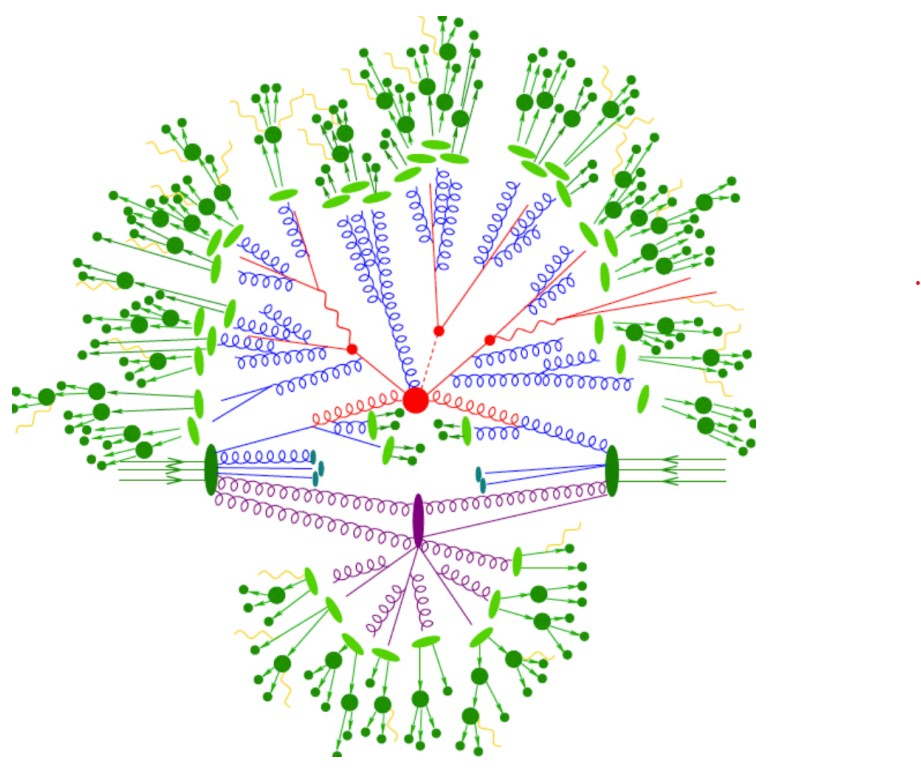
\includegraphics[scale=0.65]{figs/ch4/mc-diagram.jpg}
    \caption{ Illustration of a hadron-hadron collision simulated by a MC generator. The center red circle signifies the hard scatter collision while the purple oval represents underlying soft-scatter events. The red and blue tree-like structures depict QCD bremsstrahlung simulated by parton showering. The other elements are hadronization (light green), hadron decays (dark green), and photon radiation (yellow). \cite{parton-showering}}
\label{fig:mc-diagram}
\end{figure}
